\documentclass{article}

\usepackage{graphicx}
\usepackage{rotating}
\usepackage{amsmath}
\usepackage{amssymb}
\usepackage{fancyhdr}
\usepackage{listings}
%\usepackage{xcolor}
\usepackage{color}
\usepackage{amsfonts}
\usepackage{textcomp}
\usepackage{float}
\usepackage[sorting=none]{biblatex}
\usepackage[margin=1in]{geometry}
\usepackage[font={small,it}]{caption}
\usepackage[table,xcdraw]{xcolor}
\usepackage{placeins}
\usepackage{xepersian}





%\DeclareMathOperator*{\btie}{\bowtie}
\addbibresource{bibliography.bib}
\settextfont[Scale=1.2]{B-NAZANIN.TTF}
\setlatintextfont[Scale=1]{Times New Roman}
\renewcommand{\baselinestretch}{1.5}
\pagestyle{fancy}
\fancyhf{}
\rhead{تکلیف اول درس مبانی رمزنگاری}
\lhead{\thepage}
\rfoot{علیرضا ابره فروش}
\lfoot{9816603}
\renewcommand{\headrulewidth}{1pt}
\renewcommand{\footrulewidth}{1pt}
%%%%%%%%%%
\lstset
{
    language=[latex]tex,
    basicstyle=\ttfamily,
    commentstyle=\color{black},
    columns=fullflexible,
    keepspaces=true,
    upquote=true,
    showstringspaces=false,
    morestring=[s]\\\%,
    stringstyle=\color{black},
}
%%%%%%%%%%
%beginMatlab
\definecolor{mygreen}{RGB}{28,172,0} % color values Red, Green, Blue
\definecolor{mylilas}{RGB}{170,55,241}
%endMatlab
\begin{document}
%beginMatlab
\lstset{language=Matlab,%
    %basicstyle=\color{red},
    breaklines=true,%
    morekeywords={matlab2tikz},
    keywordstyle=\color{blue},%
    morekeywords=[2]{1}, keywordstyle=[2]{\color{black}},
    identifierstyle=\color{black},%
    stringstyle=\color{mylilas},
    commentstyle=\color{mygreen},%
    showstringspaces=false,%without this there will be a symbol in the places where there is a space
    numbers=left,%
    numberstyle={\tiny \color{black}},% size of the numbers
    numbersep=9pt, % this defines how far the numbers are from the text
    emph=[1]{for,end,break},emphstyle=[1]\color{red}, %some words to emphasise
    %emph=[2]{word1,word2}, emphstyle=[2]{style},    
}
%endMatlab
\begin{titlepage}
\begin{center}

\includegraphics[width=0.4\textwidth]{figures/IUT Logo.png}\\
        
\LARGE
\textbf{دانشگاه صنعتی اصفهان}\\
\textbf{دانشکده مهندسی برق و کامپیوتر}\\
        
\vfill
        
\huge
\textbf{عنوان: تکلیف چهارم درس ریزپردازنده}\\
        
\vfill
        
\LARGE
\textbf{نام و نام خانوادگی: علیرضا ابره فروش}\\
\textbf{شماره دانشجویی: 9816603}\\
\textbf{نیم\,سال تحصیلی: پاییز 1400}\\
\textbf{مدرّس: دکتر عارف کریمی افشار}\\
\end{center}
\end{titlepage}


%\tableofcontents
\newpage


\section{}%1
\subsection{\lr{a}}
کلید \lr{Caesar cipher} برابر \lr{M} است که حرف 13ام الفبای انگلیسی است. پس در واقع هر حرفِ الفبا به صورت حلقوی 12 واحد شیفت می‌خورد. پس در نهایت به صورت زیر رمز می‌شود.
\begin{latin}
% Please add the following required packages to your document preamble:
% \usepackage{graphicx}
\begin{table}[H]
\centering
\resizebox{\columnwidth}{!}{%
\begin{tabular}{|c|c|c|c|c|c|c|c|c|c|c|c|c|c|c|c|c|c|c|c|c|}
\hline
x           & A & l & i & r & e & z & a &  & A & b & r & e & h & f & o & r & o & u & s & h \\ \hline
$E_{12}(x)$ & M & x & u & d & q & l & m &  & M & n & d & q & t & r & a & d & a & g & e & t \\ \hline
\end{tabular}%
}
\end{table}
\end{latin}
در نرم افزار \lr{CrypTool} به صورت زیر رمز می‌کنیم.
\begin{figure}[H]
    \centering
    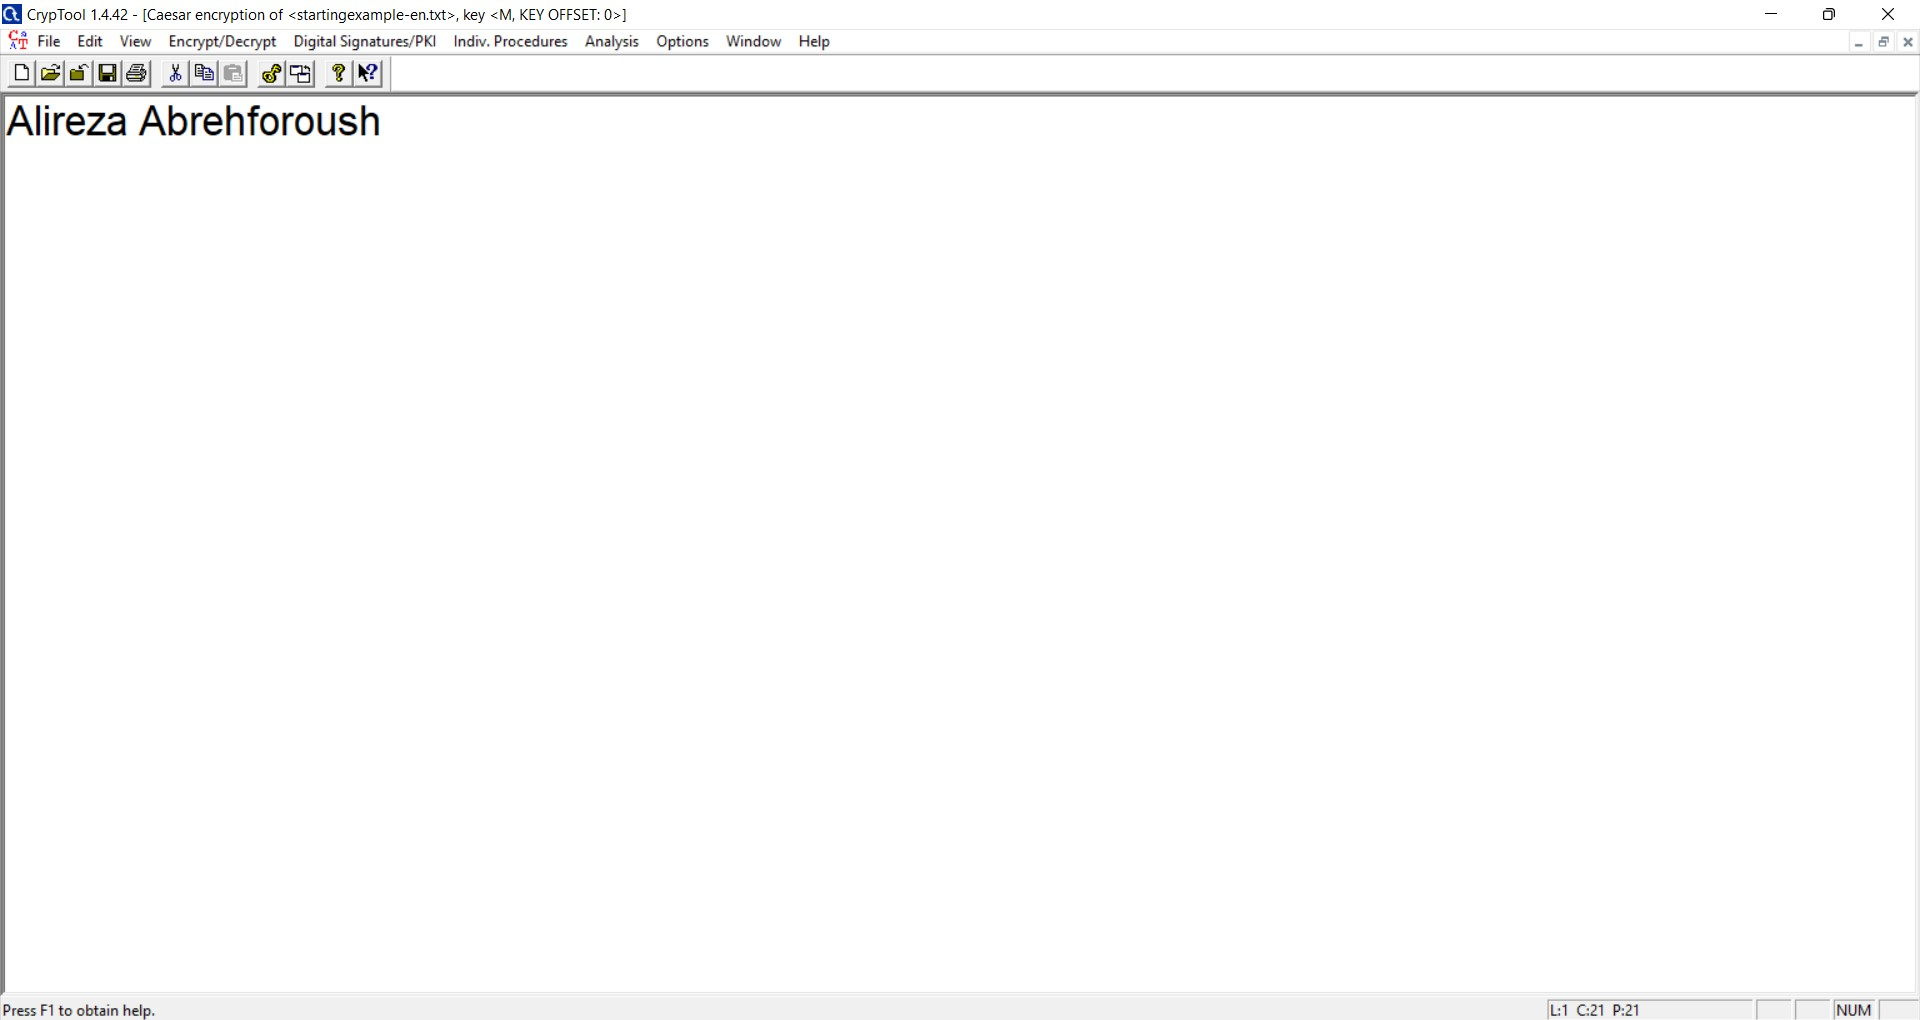
\includegraphics[width=0.75\textwidth]{figures/1a.jpg}
    \caption
	{}
    \label{fig:fig1}
\end{figure}

\begin{figure}[H]
    \centering
    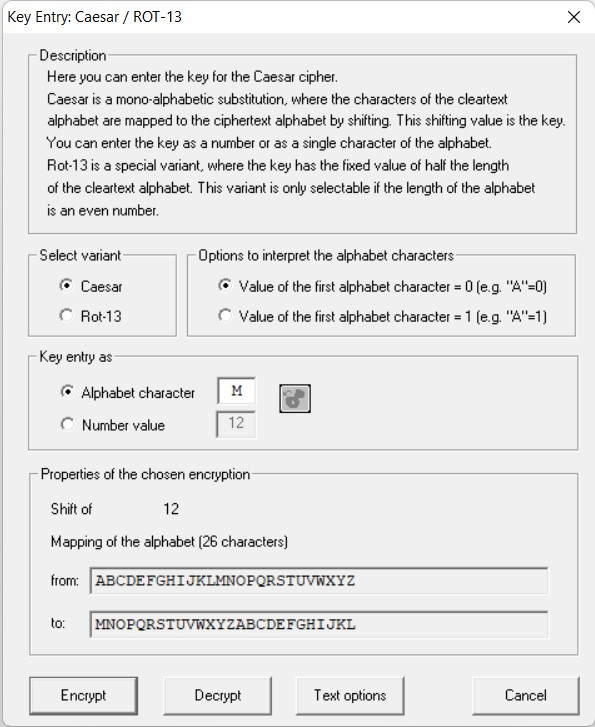
\includegraphics[width=0.25\textwidth]{figures/1b.jpg}
    \caption
	{}
    \label{fig:fig1}
\end{figure}

\begin{figure}[H]
    \centering
    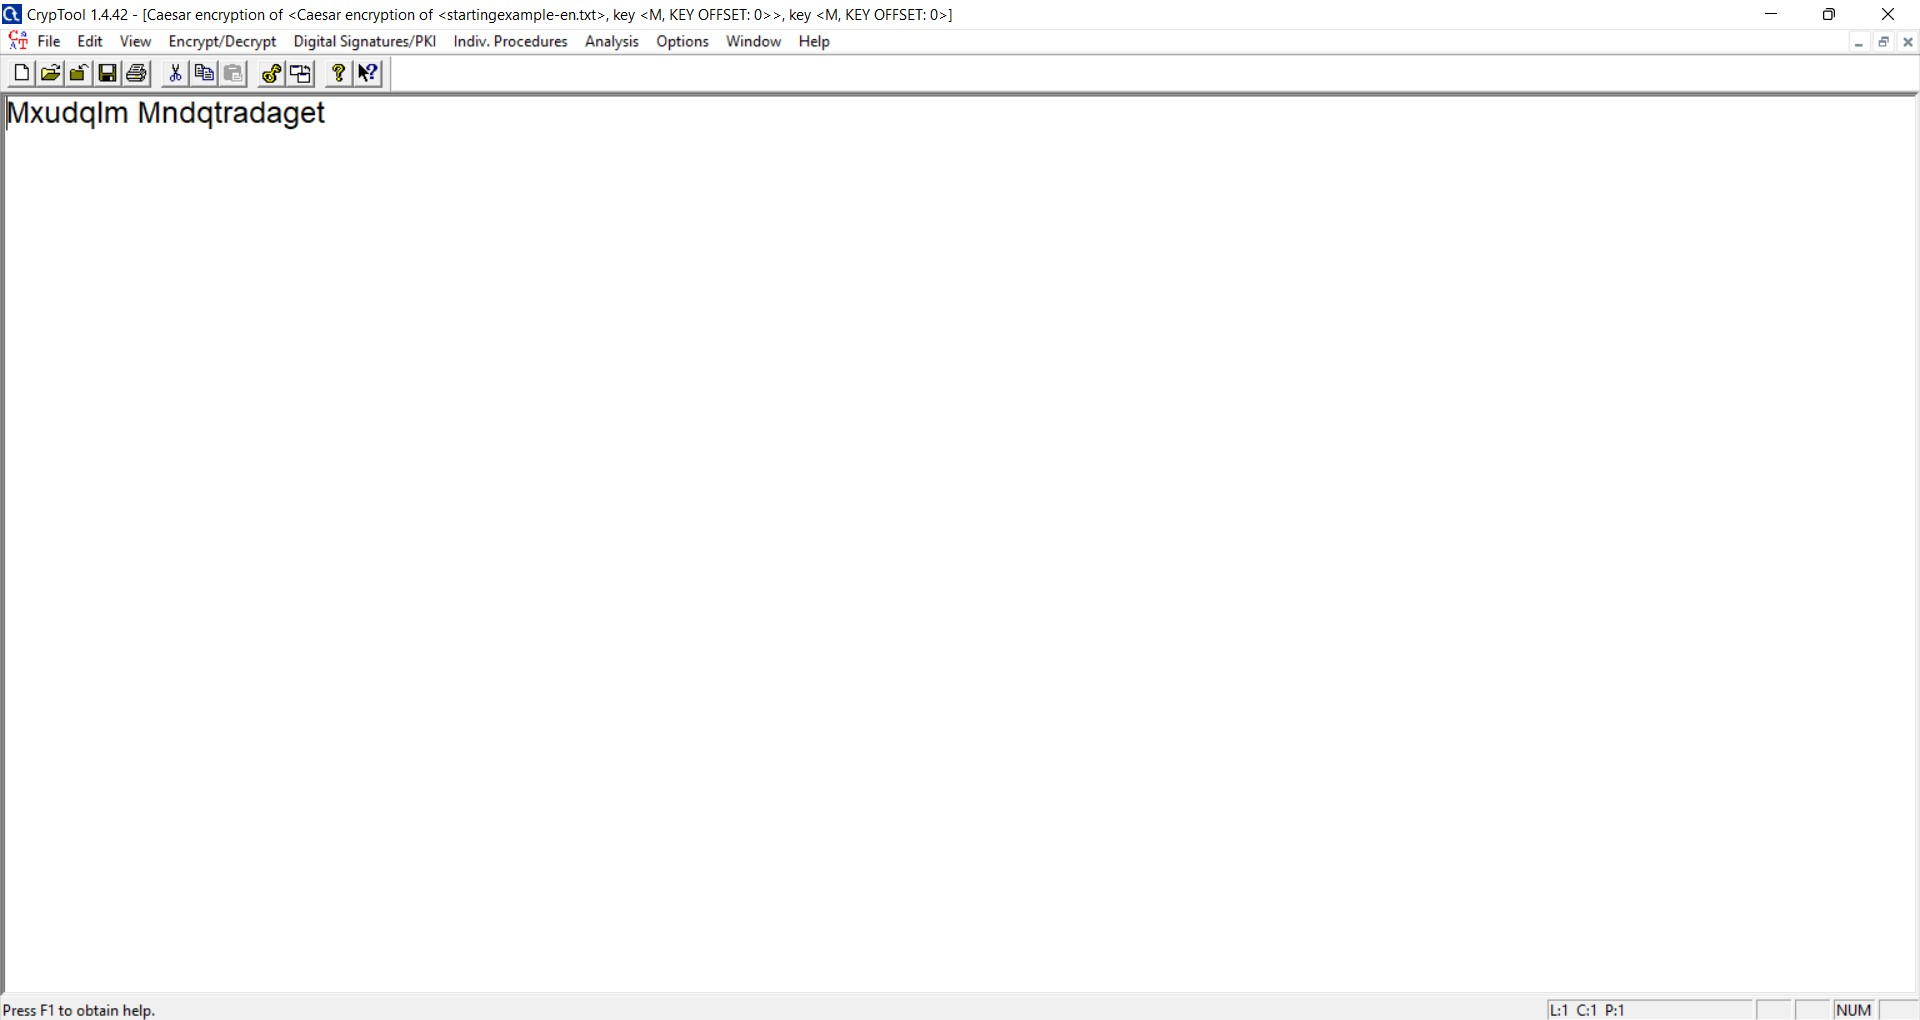
\includegraphics[width=0.75\textwidth]{figures/1c.jpg}
    \caption
	{}
    \label{fig:fig1}
\end{figure}

\section{}%2
\begin{latin}
$
9816603 \equiv 17 \:\:\:\:mod\:\: 26
$
\end{latin}
کلید \lr{Substitution cipher} برابر \lr{fharjolyinectzspdbkwxgumvq} و \lr{offset} آن برابر 17 است. در واقع الفبای اگلیسی به ترتیب به \lr{NECTZSPDBKWXGUMVQFHARJOLYI} \lr{map} می‌شود. پس در نهایت به صورت زیر رمز می‌شود.
\begin{latin}
% Please add the following required packages to your document preamble:
% \usepackage{graphicx}
\begin{table}[H]
\centering
\resizebox{\columnwidth}{!}{%
\begin{tabular}{|c|c|c|c|c|c|c|c|c|c|c|c|c|c|c|c|c|c|c|c|c|c|c|c|c|c|c|c|c|c|c|c|c|c|c|c|c|c|c|c|c|c|c|c|c|c|c|c|c|c|c|c|c|c|c|c|c|c|c|c|c|c|c|c|c|c|c|c|c|c|}
\hline
x           & S & u & c & c & e & s & s &  & u & s & u & a & l & l & y &  & c & o & m & e & s &  & t & o &  & t & h & o & s & e &  & w & h & o &  & a & r & e &  & t & o & o &  & b & u & s & y &  & t & o &  & b & e &  & l & o & o & k & i & n & g &  & f & o & r &  & i & t & . \\ \hline
$E(x)$ & H & r & c & c & z & h & h &  & r & h & r & n & x & x & y &  & c & m & g & z & h &  & a & m &  & a & d & m & h & z &  & o & d & m &  & n & f & z &  & a & m & m &  & e & r & h & y &  & a & m &  & e & z &  & x & m & m & w & b & u & p &  & s & m & f &  & b & a & . \\ \hline
\end{tabular}%
}
\end{table}
\end{latin}
در نرم افزار \lr{CrypTool} به صورت زیر رمز می‌کنیم.
\begin{figure}[H]
    \centering
    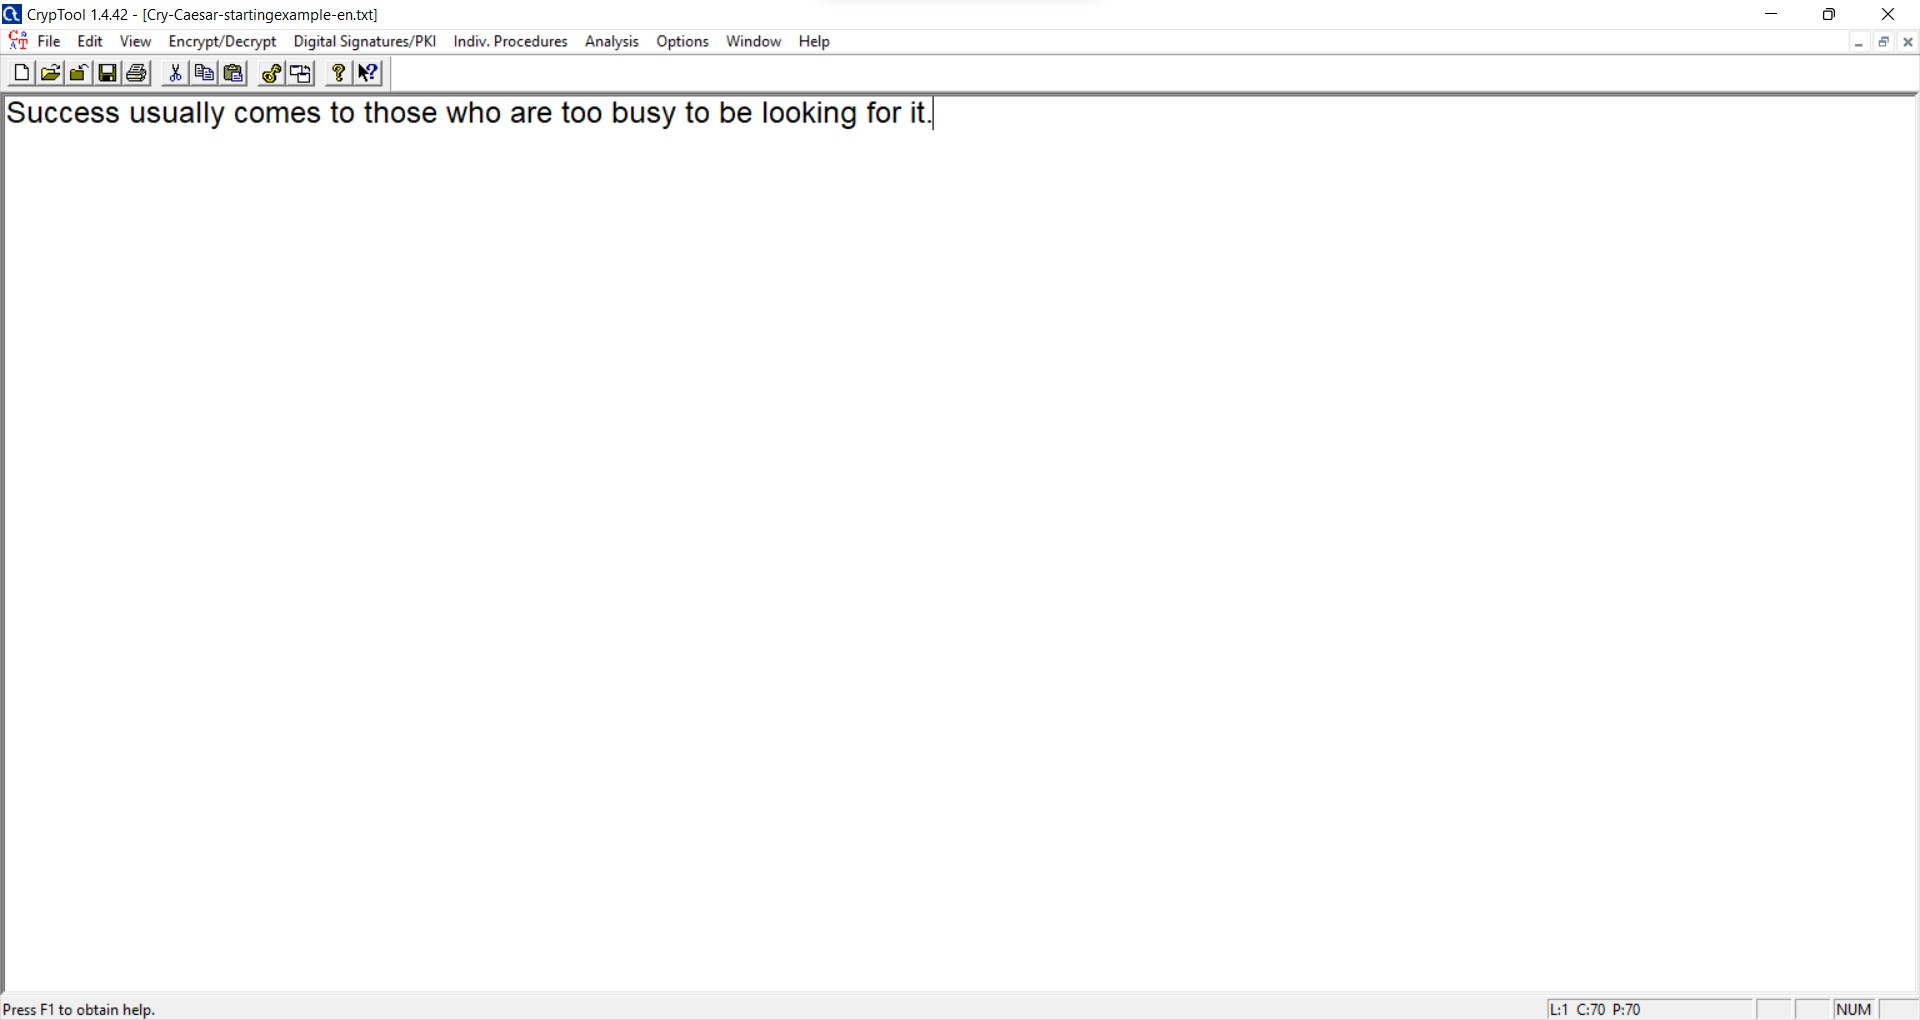
\includegraphics[width=0.75\textwidth]{figures/2a.jpg}
    \caption
	{}
    \label{fig:fig1}
\end{figure}

\begin{figure}[H]
    \centering
    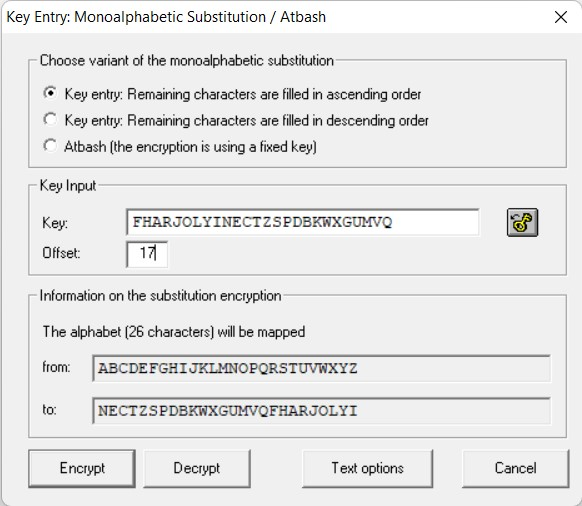
\includegraphics[width=0.25\textwidth]{figures/2b.jpg}
    \caption
	{}
    \label{fig:fig1}
\end{figure}

\begin{figure}[H]
    \centering
    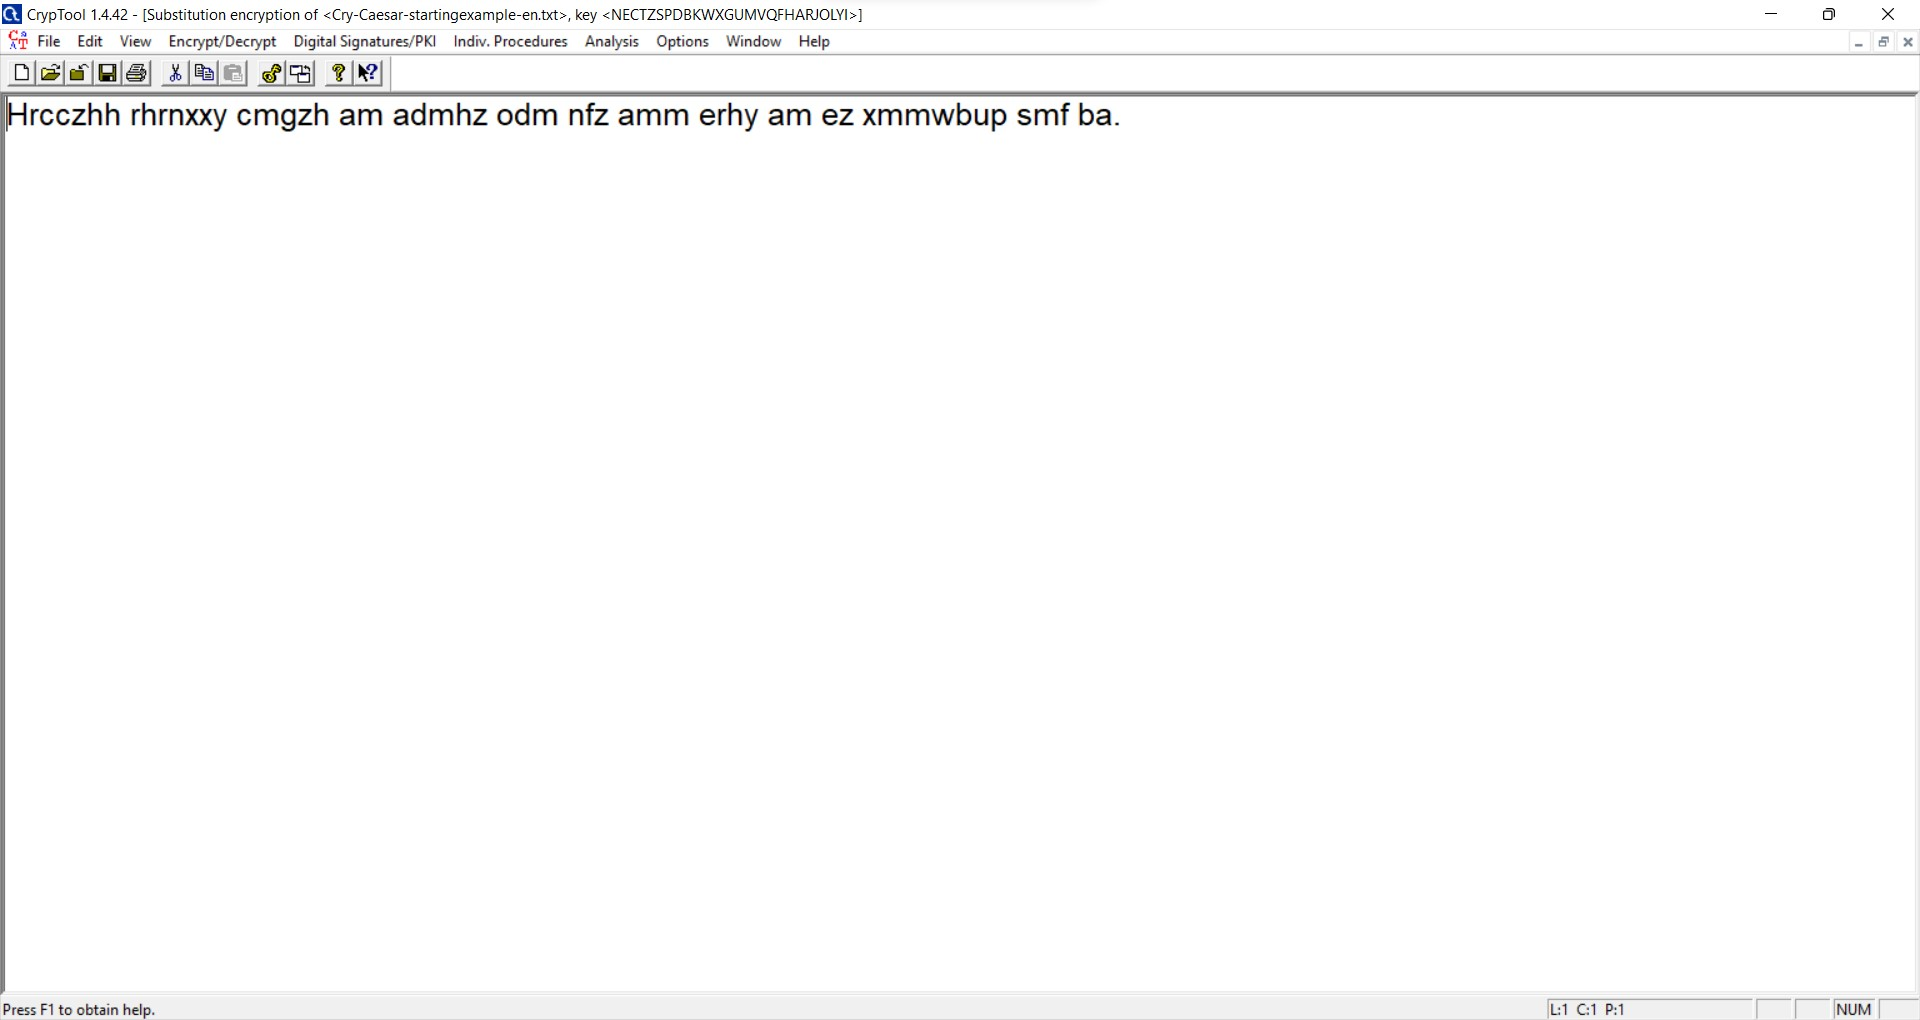
\includegraphics[width=0.75\textwidth]{figures/2c.jpg}
    \caption
	{}
    \label{fig:fig1}
\end{figure}


\section{}%3
\subsection{\lr{a}}
در \lr{Vigenère cipher} در الفبای انگلیسی از یک جدول با ابعاد $26 \times 26$ استفاده می‌شود که در سطر $i$ام آن حروف انگلیسی به ترتیب به صورت حلقوی با شروع از حرف $i$ام الفبا نوشته شده است.
\begin{latin}
% Please add the following required packages to your document preamble:
% \usepackage{graphicx}
\begin{table}[H]
\centering
\resizebox{\columnwidth}{!}{%
\begin{tabular}{ccccccccccccccccccccccccccc}
                                & \textbf{A}             & \textbf{B}             & \textbf{C}             & \textbf{D}             & \textbf{E}             & \textbf{F}             & \textbf{G}             & \textbf{H}             & \textbf{I}             & \textbf{J}             & \textbf{K}             & \textbf{L}             & \textbf{M}             & \textbf{N}             & \textbf{O}             & \textbf{P}             & \textbf{Q}             & \textbf{R}             & \textbf{S}             & \textbf{T}             & \textbf{U}             & \textbf{V}             & \textbf{W}             & \textbf{X}             & \textbf{Y}             & \textbf{Z}             \\ \cline{2-27} 
\multicolumn{1}{c|}{\textbf{A}} & \multicolumn{1}{c|}{A} & \multicolumn{1}{c|}{B} & \multicolumn{1}{c|}{C} & \multicolumn{1}{c|}{D} & \multicolumn{1}{c|}{E} & \multicolumn{1}{c|}{F} & \multicolumn{1}{c|}{G} & \multicolumn{1}{c|}{H} & \multicolumn{1}{c|}{I} & \multicolumn{1}{c|}{J} & \multicolumn{1}{c|}{K} & \multicolumn{1}{c|}{L} & \multicolumn{1}{c|}{M} & \multicolumn{1}{c|}{N} & \multicolumn{1}{c|}{O} & \multicolumn{1}{c|}{P} & \multicolumn{1}{c|}{Q} & \multicolumn{1}{c|}{R} & \multicolumn{1}{c|}{S} & \multicolumn{1}{c|}{T} & \multicolumn{1}{c|}{U} & \multicolumn{1}{c|}{V} & \multicolumn{1}{c|}{W} & \multicolumn{1}{c|}{X} & \multicolumn{1}{c|}{Y} & \multicolumn{1}{c|}{Z} \\ \cline{2-27} 
\multicolumn{1}{c|}{\textbf{B}} & \multicolumn{1}{c|}{B} & \multicolumn{1}{c|}{C} & \multicolumn{1}{c|}{D} & \multicolumn{1}{c|}{E} & \multicolumn{1}{c|}{F} & \multicolumn{1}{c|}{G} & \multicolumn{1}{c|}{H} & \multicolumn{1}{c|}{I} & \multicolumn{1}{c|}{J} & \multicolumn{1}{c|}{K} & \multicolumn{1}{c|}{L} & \multicolumn{1}{c|}{M} & \multicolumn{1}{c|}{N} & \multicolumn{1}{c|}{O} & \multicolumn{1}{c|}{P} & \multicolumn{1}{c|}{Q} & \multicolumn{1}{c|}{R} & \multicolumn{1}{c|}{S} & \multicolumn{1}{c|}{T} & \multicolumn{1}{c|}{U} & \multicolumn{1}{c|}{V} & \multicolumn{1}{c|}{W} & \multicolumn{1}{c|}{X} & \multicolumn{1}{c|}{Y} & \multicolumn{1}{c|}{Z} & \multicolumn{1}{c|}{A} \\ \cline{2-27} 
\multicolumn{1}{c|}{\textbf{C}} & \multicolumn{1}{c|}{C} & \multicolumn{1}{c|}{D} & \multicolumn{1}{c|}{E} & \multicolumn{1}{c|}{F} & \multicolumn{1}{c|}{G} & \multicolumn{1}{c|}{H} & \multicolumn{1}{c|}{I} & \multicolumn{1}{c|}{J} & \multicolumn{1}{c|}{K} & \multicolumn{1}{c|}{L} & \multicolumn{1}{c|}{M} & \multicolumn{1}{c|}{N} & \multicolumn{1}{c|}{O} & \multicolumn{1}{c|}{P} & \multicolumn{1}{c|}{Q} & \multicolumn{1}{c|}{R} & \multicolumn{1}{c|}{S} & \multicolumn{1}{c|}{T} & \multicolumn{1}{c|}{U} & \multicolumn{1}{c|}{V} & \multicolumn{1}{c|}{W} & \multicolumn{1}{c|}{X} & \multicolumn{1}{c|}{Y} & \multicolumn{1}{c|}{Z} & \multicolumn{1}{c|}{A} & \multicolumn{1}{c|}{B} \\ \cline{2-27} 
\multicolumn{1}{c|}{\textbf{D}} & \multicolumn{1}{c|}{D} & \multicolumn{1}{c|}{E} & \multicolumn{1}{c|}{F} & \multicolumn{1}{c|}{G} & \multicolumn{1}{c|}{H} & \multicolumn{1}{c|}{I} & \multicolumn{1}{c|}{J} & \multicolumn{1}{c|}{K} & \multicolumn{1}{c|}{L} & \multicolumn{1}{c|}{M} & \multicolumn{1}{c|}{N} & \multicolumn{1}{c|}{O} & \multicolumn{1}{c|}{P} & \multicolumn{1}{c|}{Q} & \multicolumn{1}{c|}{R} & \multicolumn{1}{c|}{S} & \multicolumn{1}{c|}{T} & \multicolumn{1}{c|}{U} & \multicolumn{1}{c|}{V} & \multicolumn{1}{c|}{W} & \multicolumn{1}{c|}{X} & \multicolumn{1}{c|}{Y} & \multicolumn{1}{c|}{Z} & \multicolumn{1}{c|}{A} & \multicolumn{1}{c|}{B} & \multicolumn{1}{c|}{C} \\ \cline{2-27} 
\multicolumn{1}{c|}{\textbf{E}} & \multicolumn{1}{c|}{E} & \multicolumn{1}{c|}{F} & \multicolumn{1}{c|}{G} & \multicolumn{1}{c|}{H} & \multicolumn{1}{c|}{I} & \multicolumn{1}{c|}{J} & \multicolumn{1}{c|}{K} & \multicolumn{1}{c|}{L} & \multicolumn{1}{c|}{M} & \multicolumn{1}{c|}{N} & \multicolumn{1}{c|}{O} & \multicolumn{1}{c|}{P} & \multicolumn{1}{c|}{Q} & \multicolumn{1}{c|}{R} & \multicolumn{1}{c|}{S} & \multicolumn{1}{c|}{T} & \multicolumn{1}{c|}{U} & \multicolumn{1}{c|}{V} & \multicolumn{1}{c|}{W} & \multicolumn{1}{c|}{X} & \multicolumn{1}{c|}{Y} & \multicolumn{1}{c|}{Z} & \multicolumn{1}{c|}{A} & \multicolumn{1}{c|}{B} & \multicolumn{1}{c|}{C} & \multicolumn{1}{c|}{D} \\ \cline{2-27} 
\multicolumn{1}{c|}{\textbf{F}} & \multicolumn{1}{c|}{F} & \multicolumn{1}{c|}{G} & \multicolumn{1}{c|}{H} & \multicolumn{1}{c|}{I} & \multicolumn{1}{c|}{J} & \multicolumn{1}{c|}{K} & \multicolumn{1}{c|}{L} & \multicolumn{1}{c|}{M} & \multicolumn{1}{c|}{N} & \multicolumn{1}{c|}{O} & \multicolumn{1}{c|}{P} & \multicolumn{1}{c|}{Q} & \multicolumn{1}{c|}{R} & \multicolumn{1}{c|}{S} & \multicolumn{1}{c|}{T} & \multicolumn{1}{c|}{U} & \multicolumn{1}{c|}{V} & \multicolumn{1}{c|}{W} & \multicolumn{1}{c|}{X} & \multicolumn{1}{c|}{Y} & \multicolumn{1}{c|}{Z} & \multicolumn{1}{c|}{A} & \multicolumn{1}{c|}{B} & \multicolumn{1}{c|}{C} & \multicolumn{1}{c|}{D} & \multicolumn{1}{c|}{E} \\ \cline{2-27} 
\multicolumn{1}{c|}{\textbf{G}} & \multicolumn{1}{c|}{G} & \multicolumn{1}{c|}{H} & \multicolumn{1}{c|}{I} & \multicolumn{1}{c|}{J} & \multicolumn{1}{c|}{K} & \multicolumn{1}{c|}{L} & \multicolumn{1}{c|}{M} & \multicolumn{1}{c|}{N} & \multicolumn{1}{c|}{O} & \multicolumn{1}{c|}{P} & \multicolumn{1}{c|}{Q} & \multicolumn{1}{c|}{R} & \multicolumn{1}{c|}{S} & \multicolumn{1}{c|}{T} & \multicolumn{1}{c|}{U} & \multicolumn{1}{c|}{V} & \multicolumn{1}{c|}{W} & \multicolumn{1}{c|}{X} & \multicolumn{1}{c|}{Y} & \multicolumn{1}{c|}{Z} & \multicolumn{1}{c|}{A} & \multicolumn{1}{c|}{B} & \multicolumn{1}{c|}{C} & \multicolumn{1}{c|}{D} & \multicolumn{1}{c|}{E} & \multicolumn{1}{c|}{F} \\ \cline{2-27} 
\multicolumn{1}{c|}{\textbf{H}} & \multicolumn{1}{c|}{H} & \multicolumn{1}{c|}{I} & \multicolumn{1}{c|}{J} & \multicolumn{1}{c|}{K} & \multicolumn{1}{c|}{L} & \multicolumn{1}{c|}{M} & \multicolumn{1}{c|}{N} & \multicolumn{1}{c|}{O} & \multicolumn{1}{c|}{P} & \multicolumn{1}{c|}{Q} & \multicolumn{1}{c|}{R} & \multicolumn{1}{c|}{S} & \multicolumn{1}{c|}{T} & \multicolumn{1}{c|}{U} & \multicolumn{1}{c|}{V} & \multicolumn{1}{c|}{W} & \multicolumn{1}{c|}{X} & \multicolumn{1}{c|}{Y} & \multicolumn{1}{c|}{Z} & \multicolumn{1}{c|}{A} & \multicolumn{1}{c|}{B} & \multicolumn{1}{c|}{C} & \multicolumn{1}{c|}{D} & \multicolumn{1}{c|}{E} & \multicolumn{1}{c|}{F} & \multicolumn{1}{c|}{G} \\ \cline{2-27} 
\multicolumn{1}{c|}{\textbf{I}} & \multicolumn{1}{c|}{I} & \multicolumn{1}{c|}{J} & \multicolumn{1}{c|}{K} & \multicolumn{1}{c|}{L} & \multicolumn{1}{c|}{M} & \multicolumn{1}{c|}{N} & \multicolumn{1}{c|}{O} & \multicolumn{1}{c|}{P} & \multicolumn{1}{c|}{Q} & \multicolumn{1}{c|}{R} & \multicolumn{1}{c|}{S} & \multicolumn{1}{c|}{T} & \multicolumn{1}{c|}{U} & \multicolumn{1}{c|}{V} & \multicolumn{1}{c|}{W} & \multicolumn{1}{c|}{X} & \multicolumn{1}{c|}{Y} & \multicolumn{1}{c|}{Z} & \multicolumn{1}{c|}{A} & \multicolumn{1}{c|}{B} & \multicolumn{1}{c|}{C} & \multicolumn{1}{c|}{D} & \multicolumn{1}{c|}{E} & \multicolumn{1}{c|}{F} & \multicolumn{1}{c|}{G} & \multicolumn{1}{c|}{H} \\ \cline{2-27} 
\multicolumn{1}{c|}{\textbf{J}} & \multicolumn{1}{c|}{J} & \multicolumn{1}{c|}{K} & \multicolumn{1}{c|}{L} & \multicolumn{1}{c|}{M} & \multicolumn{1}{c|}{N} & \multicolumn{1}{c|}{O} & \multicolumn{1}{c|}{P} & \multicolumn{1}{c|}{Q} & \multicolumn{1}{c|}{R} & \multicolumn{1}{c|}{S} & \multicolumn{1}{c|}{T} & \multicolumn{1}{c|}{U} & \multicolumn{1}{c|}{V} & \multicolumn{1}{c|}{W} & \multicolumn{1}{c|}{X} & \multicolumn{1}{c|}{Y} & \multicolumn{1}{c|}{Z} & \multicolumn{1}{c|}{A} & \multicolumn{1}{c|}{B} & \multicolumn{1}{c|}{C} & \multicolumn{1}{c|}{D} & \multicolumn{1}{c|}{E} & \multicolumn{1}{c|}{F} & \multicolumn{1}{c|}{G} & \multicolumn{1}{c|}{H} & \multicolumn{1}{c|}{I} \\ \cline{2-27} 
\multicolumn{1}{c|}{\textbf{K}} & \multicolumn{1}{c|}{K} & \multicolumn{1}{c|}{L} & \multicolumn{1}{c|}{M} & \multicolumn{1}{c|}{N} & \multicolumn{1}{c|}{O} & \multicolumn{1}{c|}{P} & \multicolumn{1}{c|}{Q} & \multicolumn{1}{c|}{R} & \multicolumn{1}{c|}{S} & \multicolumn{1}{c|}{T} & \multicolumn{1}{c|}{U} & \multicolumn{1}{c|}{V} & \multicolumn{1}{c|}{W} & \multicolumn{1}{c|}{X} & \multicolumn{1}{c|}{Y} & \multicolumn{1}{c|}{Z} & \multicolumn{1}{c|}{A} & \multicolumn{1}{c|}{B} & \multicolumn{1}{c|}{C} & \multicolumn{1}{c|}{D} & \multicolumn{1}{c|}{E} & \multicolumn{1}{c|}{F} & \multicolumn{1}{c|}{G} & \multicolumn{1}{c|}{H} & \multicolumn{1}{c|}{I} & \multicolumn{1}{c|}{J} \\ \cline{2-27} 
\multicolumn{1}{c|}{\textbf{L}} & \multicolumn{1}{c|}{L} & \multicolumn{1}{c|}{M} & \multicolumn{1}{c|}{N} & \multicolumn{1}{c|}{O} & \multicolumn{1}{c|}{P} & \multicolumn{1}{c|}{Q} & \multicolumn{1}{c|}{R} & \multicolumn{1}{c|}{S} & \multicolumn{1}{c|}{T} & \multicolumn{1}{c|}{U} & \multicolumn{1}{c|}{V} & \multicolumn{1}{c|}{W} & \multicolumn{1}{c|}{X} & \multicolumn{1}{c|}{Y} & \multicolumn{1}{c|}{Z} & \multicolumn{1}{c|}{A} & \multicolumn{1}{c|}{B} & \multicolumn{1}{c|}{C} & \multicolumn{1}{c|}{D} & \multicolumn{1}{c|}{E} & \multicolumn{1}{c|}{F} & \multicolumn{1}{c|}{G} & \multicolumn{1}{c|}{H} & \multicolumn{1}{c|}{I} & \multicolumn{1}{c|}{J} & \multicolumn{1}{c|}{K} \\ \cline{2-27} 
\multicolumn{1}{c|}{\textbf{M}} & \multicolumn{1}{c|}{M} & \multicolumn{1}{c|}{N} & \multicolumn{1}{c|}{O} & \multicolumn{1}{c|}{P} & \multicolumn{1}{c|}{Q} & \multicolumn{1}{c|}{R} & \multicolumn{1}{c|}{S} & \multicolumn{1}{c|}{T} & \multicolumn{1}{c|}{U} & \multicolumn{1}{c|}{V} & \multicolumn{1}{c|}{W} & \multicolumn{1}{c|}{X} & \multicolumn{1}{c|}{Y} & \multicolumn{1}{c|}{Z} & \multicolumn{1}{c|}{A} & \multicolumn{1}{c|}{B} & \multicolumn{1}{c|}{C} & \multicolumn{1}{c|}{D} & \multicolumn{1}{c|}{E} & \multicolumn{1}{c|}{F} & \multicolumn{1}{c|}{G} & \multicolumn{1}{c|}{H} & \multicolumn{1}{c|}{I} & \multicolumn{1}{c|}{J} & \multicolumn{1}{c|}{K} & \multicolumn{1}{c|}{L} \\ \cline{2-27} 
\multicolumn{1}{c|}{\textbf{N}} & \multicolumn{1}{c|}{N} & \multicolumn{1}{c|}{O} & \multicolumn{1}{c|}{P} & \multicolumn{1}{c|}{Q} & \multicolumn{1}{c|}{R} & \multicolumn{1}{c|}{S} & \multicolumn{1}{c|}{T} & \multicolumn{1}{c|}{U} & \multicolumn{1}{c|}{V} & \multicolumn{1}{c|}{W} & \multicolumn{1}{c|}{X} & \multicolumn{1}{c|}{Y} & \multicolumn{1}{c|}{Z} & \multicolumn{1}{c|}{A} & \multicolumn{1}{c|}{B} & \multicolumn{1}{c|}{C} & \multicolumn{1}{c|}{D} & \multicolumn{1}{c|}{E} & \multicolumn{1}{c|}{F} & \multicolumn{1}{c|}{G} & \multicolumn{1}{c|}{H} & \multicolumn{1}{c|}{I} & \multicolumn{1}{c|}{J} & \multicolumn{1}{c|}{K} & \multicolumn{1}{c|}{L} & \multicolumn{1}{c|}{M} \\ \cline{2-27} 
\multicolumn{1}{c|}{\textbf{O}} & \multicolumn{1}{c|}{O} & \multicolumn{1}{c|}{P} & \multicolumn{1}{c|}{Q} & \multicolumn{1}{c|}{R} & \multicolumn{1}{c|}{S} & \multicolumn{1}{c|}{T} & \multicolumn{1}{c|}{U} & \multicolumn{1}{c|}{V} & \multicolumn{1}{c|}{W} & \multicolumn{1}{c|}{X} & \multicolumn{1}{c|}{Y} & \multicolumn{1}{c|}{Z} & \multicolumn{1}{c|}{A} & \multicolumn{1}{c|}{B} & \multicolumn{1}{c|}{C} & \multicolumn{1}{c|}{D} & \multicolumn{1}{c|}{E} & \multicolumn{1}{c|}{F} & \multicolumn{1}{c|}{G} & \multicolumn{1}{c|}{H} & \multicolumn{1}{c|}{I} & \multicolumn{1}{c|}{J} & \multicolumn{1}{c|}{K} & \multicolumn{1}{c|}{L} & \multicolumn{1}{c|}{M} & \multicolumn{1}{c|}{N} \\ \cline{2-27} 
\multicolumn{1}{c|}{\textbf{P}} & \multicolumn{1}{c|}{P} & \multicolumn{1}{c|}{Q} & \multicolumn{1}{c|}{R} & \multicolumn{1}{c|}{S} & \multicolumn{1}{c|}{T} & \multicolumn{1}{c|}{U} & \multicolumn{1}{c|}{V} & \multicolumn{1}{c|}{W} & \multicolumn{1}{c|}{X} & \multicolumn{1}{c|}{Y} & \multicolumn{1}{c|}{Z} & \multicolumn{1}{c|}{A} & \multicolumn{1}{c|}{B} & \multicolumn{1}{c|}{C} & \multicolumn{1}{c|}{D} & \multicolumn{1}{c|}{E} & \multicolumn{1}{c|}{F} & \multicolumn{1}{c|}{G} & \multicolumn{1}{c|}{H} & \multicolumn{1}{c|}{I} & \multicolumn{1}{c|}{J} & \multicolumn{1}{c|}{K} & \multicolumn{1}{c|}{L} & \multicolumn{1}{c|}{M} & \multicolumn{1}{c|}{N} & \multicolumn{1}{c|}{O} \\ \cline{2-27} 
\multicolumn{1}{c|}{\textbf{Q}} & \multicolumn{1}{c|}{Q} & \multicolumn{1}{c|}{R} & \multicolumn{1}{c|}{S} & \multicolumn{1}{c|}{T} & \multicolumn{1}{c|}{U} & \multicolumn{1}{c|}{V} & \multicolumn{1}{c|}{W} & \multicolumn{1}{c|}{X} & \multicolumn{1}{c|}{Y} & \multicolumn{1}{c|}{Z} & \multicolumn{1}{c|}{A} & \multicolumn{1}{c|}{B} & \multicolumn{1}{c|}{C} & \multicolumn{1}{c|}{D} & \multicolumn{1}{c|}{E} & \multicolumn{1}{c|}{F} & \multicolumn{1}{c|}{G} & \multicolumn{1}{c|}{H} & \multicolumn{1}{c|}{I} & \multicolumn{1}{c|}{J} & \multicolumn{1}{c|}{K} & \multicolumn{1}{c|}{L} & \multicolumn{1}{c|}{M} & \multicolumn{1}{c|}{N} & \multicolumn{1}{c|}{O} & \multicolumn{1}{c|}{P} \\ \cline{2-27} 
\multicolumn{1}{c|}{\textbf{R}} & \multicolumn{1}{c|}{R} & \multicolumn{1}{c|}{S} & \multicolumn{1}{c|}{T} & \multicolumn{1}{c|}{U} & \multicolumn{1}{c|}{V} & \multicolumn{1}{c|}{W} & \multicolumn{1}{c|}{X} & \multicolumn{1}{c|}{Y} & \multicolumn{1}{c|}{Z} & \multicolumn{1}{c|}{A} & \multicolumn{1}{c|}{B} & \multicolumn{1}{c|}{C} & \multicolumn{1}{c|}{D} & \multicolumn{1}{c|}{E} & \multicolumn{1}{c|}{F} & \multicolumn{1}{c|}{G} & \multicolumn{1}{c|}{H} & \multicolumn{1}{c|}{I} & \multicolumn{1}{c|}{J} & \multicolumn{1}{c|}{K} & \multicolumn{1}{c|}{L} & \multicolumn{1}{c|}{M} & \multicolumn{1}{c|}{N} & \multicolumn{1}{c|}{O} & \multicolumn{1}{c|}{P} & \multicolumn{1}{c|}{Q} \\ \cline{2-27} 
\multicolumn{1}{c|}{\textbf{S}} & \multicolumn{1}{c|}{S} & \multicolumn{1}{c|}{T} & \multicolumn{1}{c|}{U} & \multicolumn{1}{c|}{V} & \multicolumn{1}{c|}{W} & \multicolumn{1}{c|}{X} & \multicolumn{1}{c|}{Y} & \multicolumn{1}{c|}{Z} & \multicolumn{1}{c|}{A} & \multicolumn{1}{c|}{B} & \multicolumn{1}{c|}{C} & \multicolumn{1}{c|}{D} & \multicolumn{1}{c|}{E} & \multicolumn{1}{c|}{F} & \multicolumn{1}{c|}{G} & \multicolumn{1}{c|}{H} & \multicolumn{1}{c|}{I} & \multicolumn{1}{c|}{J} & \multicolumn{1}{c|}{K} & \multicolumn{1}{c|}{L} & \multicolumn{1}{c|}{M} & \multicolumn{1}{c|}{N} & \multicolumn{1}{c|}{O} & \multicolumn{1}{c|}{P} & \multicolumn{1}{c|}{Q} & \multicolumn{1}{c|}{R} \\ \cline{2-27} 
\multicolumn{1}{c|}{\textbf{T}} & \multicolumn{1}{c|}{T} & \multicolumn{1}{c|}{U} & \multicolumn{1}{c|}{V} & \multicolumn{1}{c|}{W} & \multicolumn{1}{c|}{X} & \multicolumn{1}{c|}{Y} & \multicolumn{1}{c|}{Z} & \multicolumn{1}{c|}{A} & \multicolumn{1}{c|}{B} & \multicolumn{1}{c|}{C} & \multicolumn{1}{c|}{D} & \multicolumn{1}{c|}{E} & \multicolumn{1}{c|}{F} & \multicolumn{1}{c|}{G} & \multicolumn{1}{c|}{H} & \multicolumn{1}{c|}{I} & \multicolumn{1}{c|}{J} & \multicolumn{1}{c|}{K} & \multicolumn{1}{c|}{L} & \multicolumn{1}{c|}{M} & \multicolumn{1}{c|}{N} & \multicolumn{1}{c|}{O} & \multicolumn{1}{c|}{P} & \multicolumn{1}{c|}{Q} & \multicolumn{1}{c|}{R} & \multicolumn{1}{c|}{S} \\ \cline{2-27} 
\multicolumn{1}{c|}{\textbf{U}} & \multicolumn{1}{c|}{U} & \multicolumn{1}{c|}{V} & \multicolumn{1}{c|}{W} & \multicolumn{1}{c|}{X} & \multicolumn{1}{c|}{Y} & \multicolumn{1}{c|}{Z} & \multicolumn{1}{c|}{A} & \multicolumn{1}{c|}{B} & \multicolumn{1}{c|}{C} & \multicolumn{1}{c|}{D} & \multicolumn{1}{c|}{E} & \multicolumn{1}{c|}{F} & \multicolumn{1}{c|}{G} & \multicolumn{1}{c|}{H} & \multicolumn{1}{c|}{I} & \multicolumn{1}{c|}{J} & \multicolumn{1}{c|}{K} & \multicolumn{1}{c|}{L} & \multicolumn{1}{c|}{M} & \multicolumn{1}{c|}{N} & \multicolumn{1}{c|}{O} & \multicolumn{1}{c|}{P} & \multicolumn{1}{c|}{Q} & \multicolumn{1}{c|}{R} & \multicolumn{1}{c|}{S} & \multicolumn{1}{c|}{T} \\ \cline{2-27} 
\multicolumn{1}{c|}{\textbf{V}} & \multicolumn{1}{c|}{V} & \multicolumn{1}{c|}{W} & \multicolumn{1}{c|}{X} & \multicolumn{1}{c|}{Y} & \multicolumn{1}{c|}{Z} & \multicolumn{1}{c|}{A} & \multicolumn{1}{c|}{B} & \multicolumn{1}{c|}{C} & \multicolumn{1}{c|}{D} & \multicolumn{1}{c|}{E} & \multicolumn{1}{c|}{F} & \multicolumn{1}{c|}{G} & \multicolumn{1}{c|}{H} & \multicolumn{1}{c|}{I} & \multicolumn{1}{c|}{J} & \multicolumn{1}{c|}{K} & \multicolumn{1}{c|}{L} & \multicolumn{1}{c|}{M} & \multicolumn{1}{c|}{N} & \multicolumn{1}{c|}{O} & \multicolumn{1}{c|}{P} & \multicolumn{1}{c|}{Q} & \multicolumn{1}{c|}{R} & \multicolumn{1}{c|}{S} & \multicolumn{1}{c|}{T} & \multicolumn{1}{c|}{U} \\ \cline{2-27} 
\multicolumn{1}{c|}{\textbf{W}} & \multicolumn{1}{c|}{W} & \multicolumn{1}{c|}{X} & \multicolumn{1}{c|}{Y} & \multicolumn{1}{c|}{Z} & \multicolumn{1}{c|}{A} & \multicolumn{1}{c|}{B} & \multicolumn{1}{c|}{C} & \multicolumn{1}{c|}{D} & \multicolumn{1}{c|}{E} & \multicolumn{1}{c|}{F} & \multicolumn{1}{c|}{G} & \multicolumn{1}{c|}{H} & \multicolumn{1}{c|}{I} & \multicolumn{1}{c|}{J} & \multicolumn{1}{c|}{K} & \multicolumn{1}{c|}{L} & \multicolumn{1}{c|}{M} & \multicolumn{1}{c|}{N} & \multicolumn{1}{c|}{O} & \multicolumn{1}{c|}{P} & \multicolumn{1}{c|}{Q} & \multicolumn{1}{c|}{R} & \multicolumn{1}{c|}{S} & \multicolumn{1}{c|}{T} & \multicolumn{1}{c|}{U} & \multicolumn{1}{c|}{V} \\ \cline{2-27} 
\multicolumn{1}{c|}{\textbf{X}} & \multicolumn{1}{c|}{X} & \multicolumn{1}{c|}{Y} & \multicolumn{1}{c|}{Z} & \multicolumn{1}{c|}{A} & \multicolumn{1}{c|}{B} & \multicolumn{1}{c|}{C} & \multicolumn{1}{c|}{D} & \multicolumn{1}{c|}{E} & \multicolumn{1}{c|}{F} & \multicolumn{1}{c|}{G} & \multicolumn{1}{c|}{H} & \multicolumn{1}{c|}{I} & \multicolumn{1}{c|}{J} & \multicolumn{1}{c|}{K} & \multicolumn{1}{c|}{L} & \multicolumn{1}{c|}{M} & \multicolumn{1}{c|}{N} & \multicolumn{1}{c|}{O} & \multicolumn{1}{c|}{P} & \multicolumn{1}{c|}{Q} & \multicolumn{1}{c|}{R} & \multicolumn{1}{c|}{S} & \multicolumn{1}{c|}{T} & \multicolumn{1}{c|}{U} & \multicolumn{1}{c|}{V} & \multicolumn{1}{c|}{W} \\ \cline{2-27} 
\multicolumn{1}{c|}{\textbf{Y}} & \multicolumn{1}{c|}{Y} & \multicolumn{1}{c|}{Z} & \multicolumn{1}{c|}{A} & \multicolumn{1}{c|}{B} & \multicolumn{1}{c|}{C} & \multicolumn{1}{c|}{D} & \multicolumn{1}{c|}{E} & \multicolumn{1}{c|}{F} & \multicolumn{1}{c|}{G} & \multicolumn{1}{c|}{H} & \multicolumn{1}{c|}{I} & \multicolumn{1}{c|}{J} & \multicolumn{1}{c|}{K} & \multicolumn{1}{c|}{L} & \multicolumn{1}{c|}{M} & \multicolumn{1}{c|}{N} & \multicolumn{1}{c|}{O} & \multicolumn{1}{c|}{P} & \multicolumn{1}{c|}{Q} & \multicolumn{1}{c|}{R} & \multicolumn{1}{c|}{S} & \multicolumn{1}{c|}{T} & \multicolumn{1}{c|}{U} & \multicolumn{1}{c|}{V} & \multicolumn{1}{c|}{W} & \multicolumn{1}{c|}{X} \\ \cline{2-27} 
\multicolumn{1}{c|}{\textbf{Z}} & \multicolumn{1}{c|}{Z} & \multicolumn{1}{c|}{A} & \multicolumn{1}{c|}{B} & \multicolumn{1}{c|}{C} & \multicolumn{1}{c|}{D} & \multicolumn{1}{c|}{E} & \multicolumn{1}{c|}{F} & \multicolumn{1}{c|}{G} & \multicolumn{1}{c|}{H} & \multicolumn{1}{c|}{I} & \multicolumn{1}{c|}{J} & \multicolumn{1}{c|}{K} & \multicolumn{1}{c|}{L} & \multicolumn{1}{c|}{M} & \multicolumn{1}{c|}{N} & \multicolumn{1}{c|}{O} & \multicolumn{1}{c|}{P} & \multicolumn{1}{c|}{Q} & \multicolumn{1}{c|}{R} & \multicolumn{1}{c|}{S} & \multicolumn{1}{c|}{T} & \multicolumn{1}{c|}{U} & \multicolumn{1}{c|}{V} & \multicolumn{1}{c|}{W} & \multicolumn{1}{c|}{X} & \multicolumn{1}{c|}{Y} \\ \cline{2-27} 
\end{tabular}%
}
\end{table}
\end{latin}
%%%%%%%%%%%%%%
همچنین کلید مورد استفاده در این الگوریتم به صورت زیر (سه حرف اول نام + سه حرف اول نام خانوادگی) ساخته می‌شود.
\begin{latin}
$
ALIREZA\:\:ABREHFOROUSH \Rightarrow key = ALIABR
$
\end{latin}
حال \lr{key} را مکررا تکرار می‌کنیم تا طول آن برابر طول رشته‌ای که می‌خواهیم آن را رمز کنیم بشود (یا به عبارتی کاراکتر نظیر باقیمانده‌ی $i$ به پیمانه‌ی طول کلید (6) را در کلید به دست آوریم). برای رمز کردن کاراکترِ $i$ام در رشته، کاراکترِ اندیسِ باقیمانده‌ی $i$ به پیمانه‌ی طول کلید (6) در کلید ($key_i$) به همراه خود کاراکترِ $i$ام ($x_i$) به دست می‌آوریم. $cipher_i$ نظیر $x_i$ برابر کاراکتر قرار گرفته در سطرِ $key_i$ و ستون $x_i$ است.
\begin{latin}
% Please add the following required packages to your document preamble:
% \usepackage{graphicx}
\begin{table}[H]
\centering
\resizebox{\columnwidth}{!}{%
\begin{tabular}{|c|c|c|c|c|c|c|c|c|c|c|c|c|c|c|c|c|c|c|c|c|c|c|c|c|c|c|c|c|c|c|c|c|c|c|c|c|c|c|c|c|c|c|c|c|c|c|c|c|c|c|c|c|c|c|c|c|c|c|c|c|c|c|c|c|c|c|c|c|c|}
\hline
key    & A & l & i & a & b & r & a &  & l & i & a & b & r & a & l &  & i & a & b & r & a &  & l & i &  & a & b & r & a & l &  & i & a & b &  & r & a & l &  & i & a & b &  & r & a & l & i &  & a & b &  & r & a &  & l & i & a & b & r & a & l &  & i & a & b &  & r & a & . \\ \hline
x      & S & u & c & c & e & s & s &  & u & s & u & a & l & l & y &  & c & o & m & e & s &  & t & o &  & t & h & o & s & e &  & w & h & o &  & a & r & e &  & t & o & o &  & b & u & s & y &  & t & o &  & b & e &  & l & o & o & k & i & n & g &  & f & o & r &  & i & t & . \\ \hline
$E(x)$ & S & f & k & c & f & j & s &  & f & a & u & b & c & l & j &  & k & o & n & v & s &  & e & w &  & t & i & f & s & p &  & e & h & p &  & r & r & p &  & b & o & p &  & s & u & d & g &  & t & p &  & s & e &  & w & w & o & l & z & n & r &  & n & o & s &  & z & t & . \\ \hline
\end{tabular}%
}
\end{table}
\end{latin}
در نرم افزار \lr{CrypTool} به صورت زیر رمز می‌کنیم.
\begin{figure}[H]
    \centering
    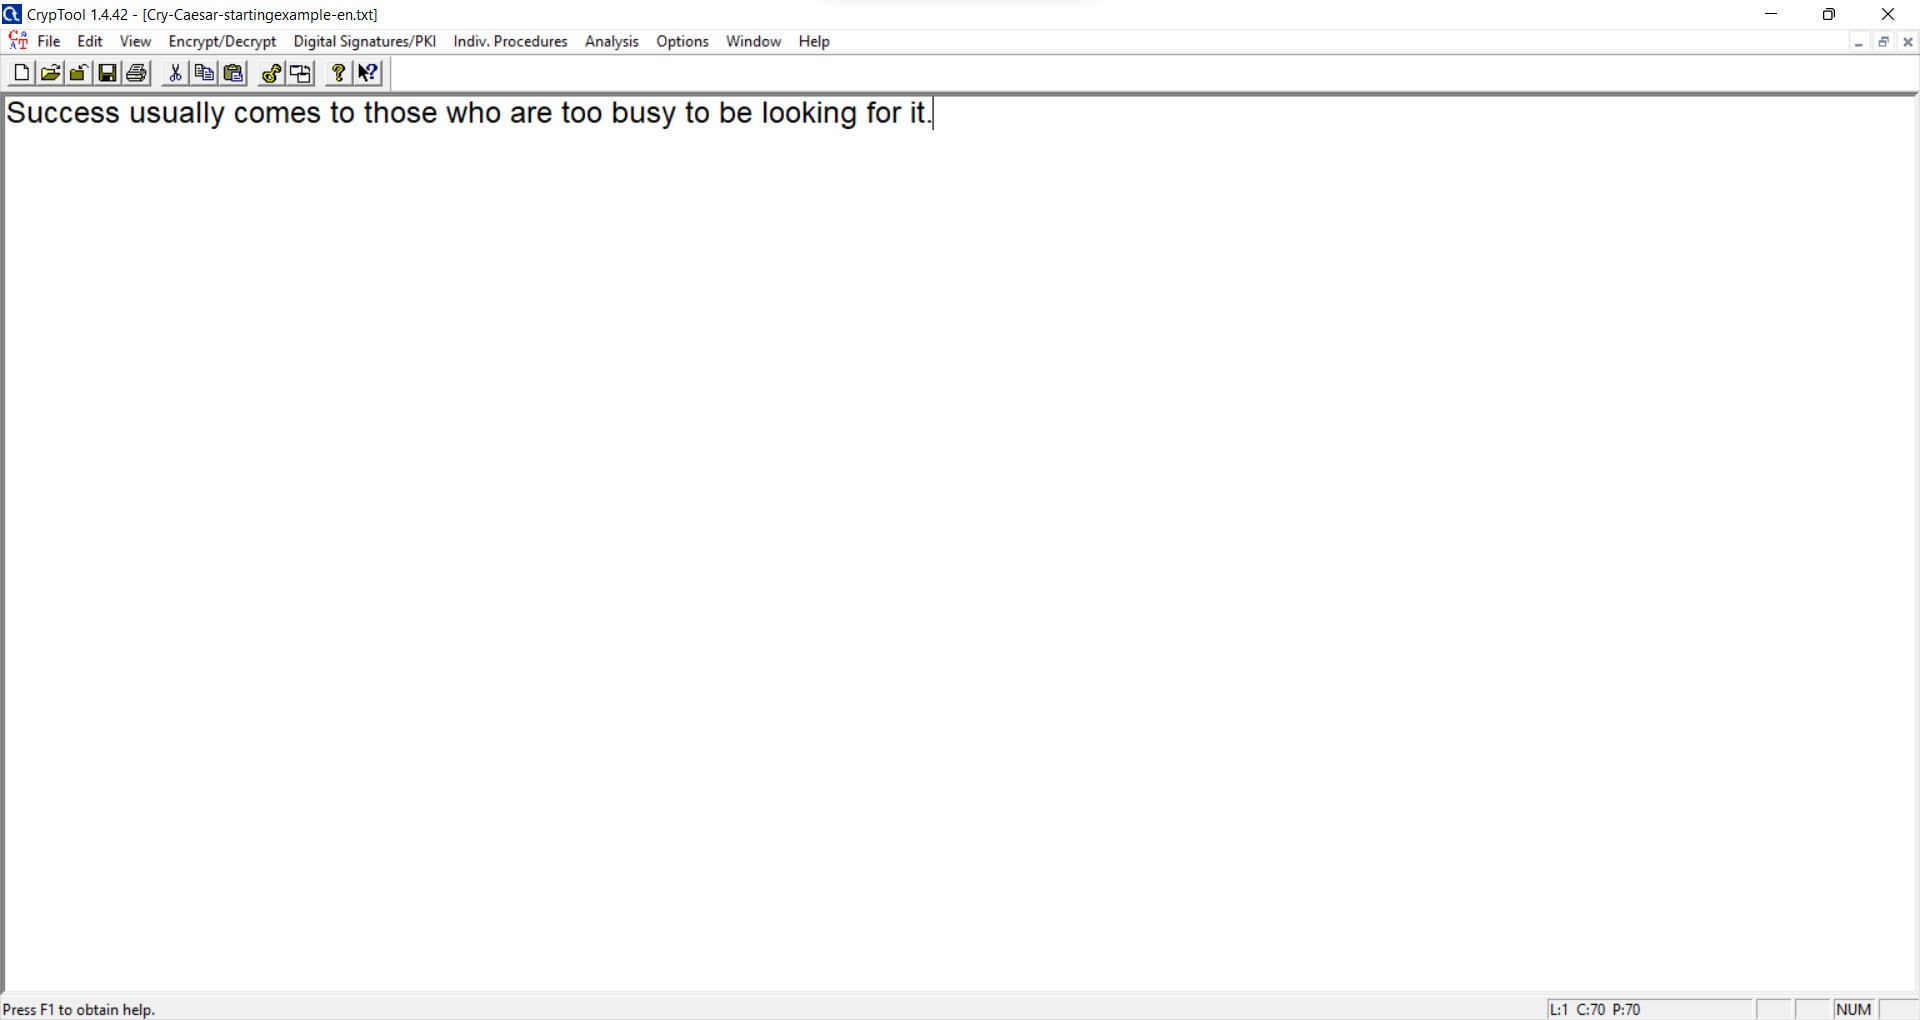
\includegraphics[width=0.75\textwidth]{figures/3aa.jpg}
    \caption
	{}
    \label{fig:fig1}
\end{figure}

\begin{figure}[H]
    \centering
    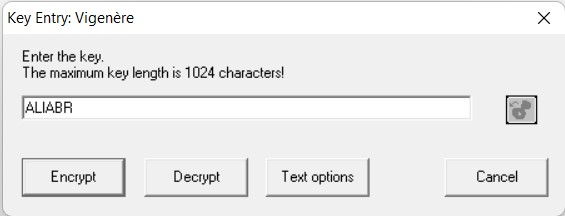
\includegraphics[width=0.25\textwidth]{figures/3ab.jpg}
    \caption
	{}
    \label{fig:fig1}
\end{figure}

\begin{figure}[H]
    \centering
    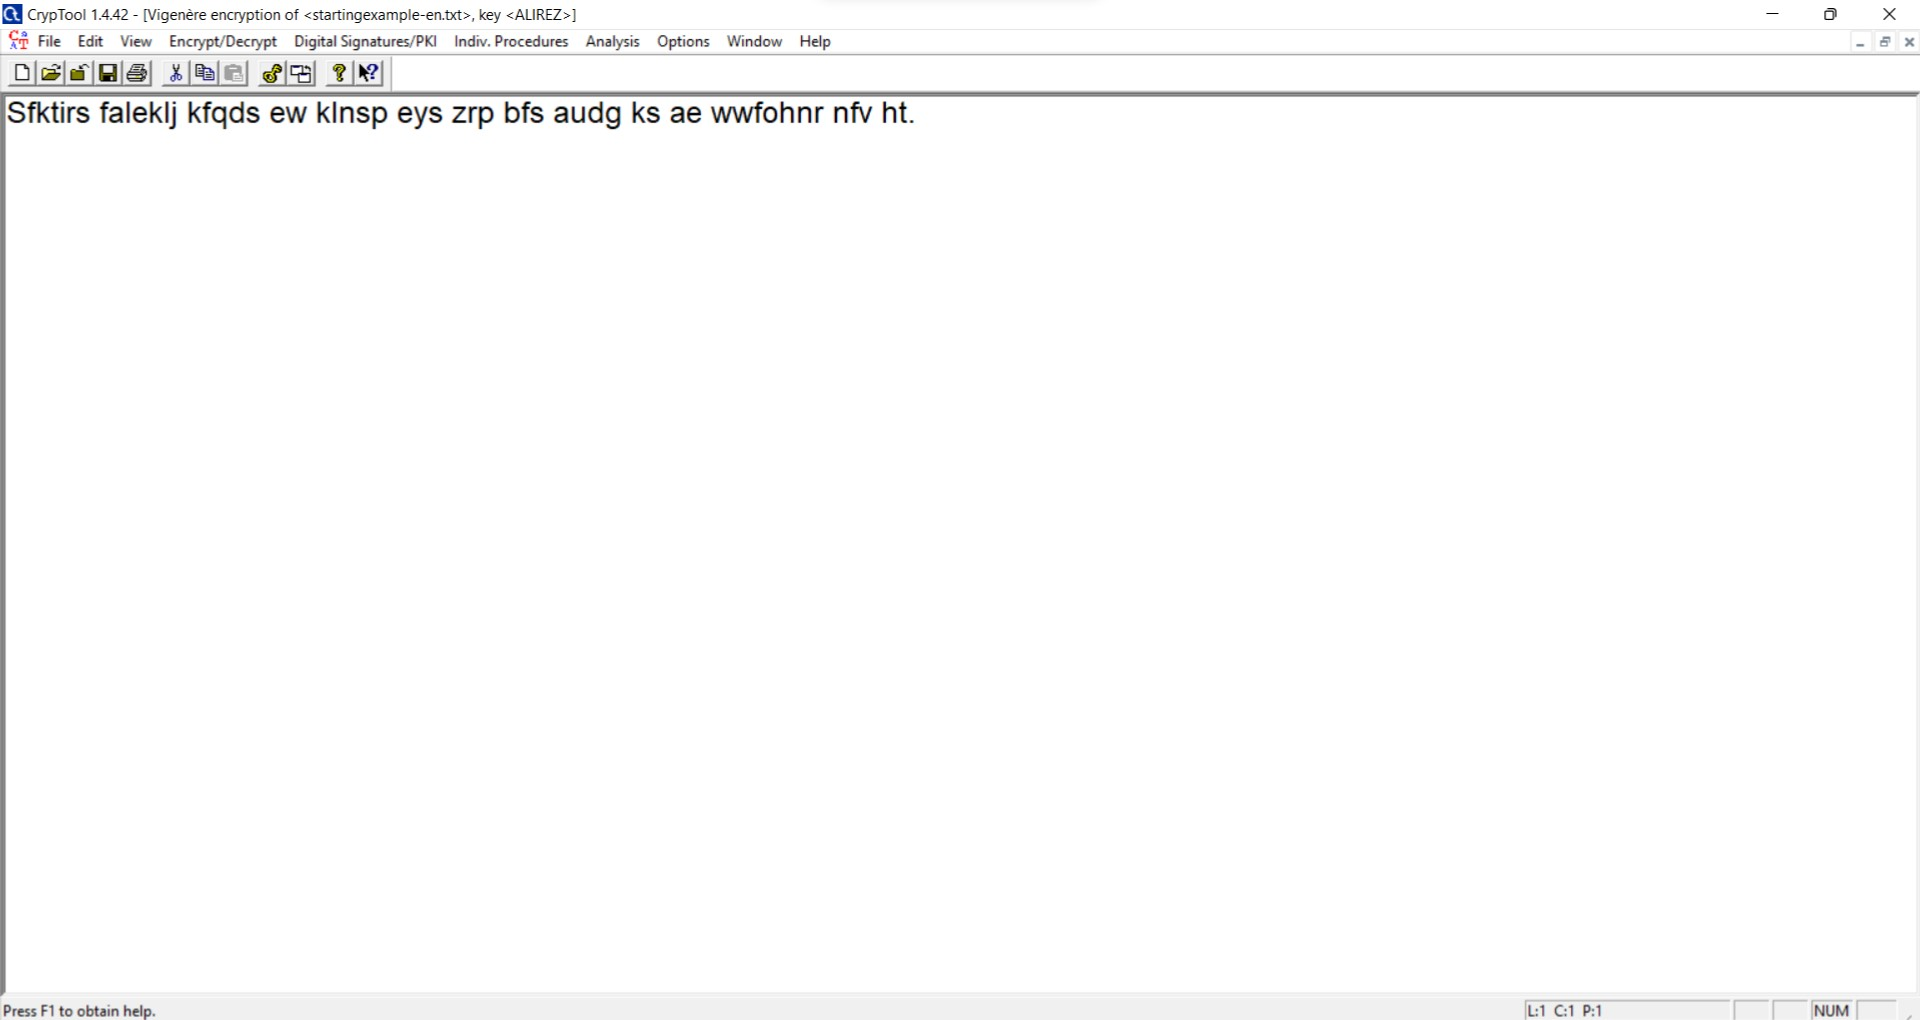
\includegraphics[width=0.75\textwidth]{figures/3ac.jpg}
    \caption
	{}
    \label{fig:fig1}
\end{figure}

\subsection{\lr{b}}
مشابه قسمت قبل (صرفا تغییر کلید) داریم:
\begin{latin}
$
ALIREZA\:\:ABREHFOROUSH \Rightarrow key = ALIREZAABREHFOROUSH
$
\end{latin}

\begin{latin}
% Please add the following required packages to your document preamble:
% \usepackage{graphicx}
\begin{table}[H]
\centering
\resizebox{\columnwidth}{!}{%
\begin{tabular}{|c|c|c|c|c|c|c|c|c|c|c|c|c|c|c|c|c|c|c|c|c|c|c|c|c|c|c|c|c|c|c|c|c|c|c|c|c|c|c|c|c|c|c|c|c|c|c|c|c|c|c|c|c|c|c|c|c|c|c|c|c|c|c|c|c|c|c|c|c|c|}
\hline
key    & A & l & i & r & e & z & a &  & a & b & r & e & h & f & o &  & r & o & u & s & h &  & a & l &  & i & r & e & z & a &  & a & b & r &  & e & h & f &  & o & r & o &  & u & s & h & a &  & l & i &  & r & e &  & z & a & a & b & r & e & h &  & f & o & r &  & o & u & . \\ \hline
x      & S & u & c & c & e & s & s &  & u & s & u & a & l & l & y &  & c & o & m & e & s &  & t & o &  & t & h & o & s & e &  & w & h & o &  & a & r & e &  & t & o & o &  & b & u & s & y &  & t & o &  & b & e &  & l & o & o & k & i & n & g &  & f & o & r &  & i & t & . \\ \hline
$E(x)$ & S & f & k & t & i & r & s &  & u & t & l & e & s & q & m &  & t & c & g & w & z &  & t & z &  & b & y & s & r & e &  & w & i & f &  & e & y & j &  & h & f & c &  & v & m & z & y &  & e & w &  & s & i &  & k & o & o & l & z & r & n &  & k & c & i &  & w & n & . \\ \hline
\end{tabular}%
}
\end{table}
\end{latin}
در نرم افزار \lr{CrypTool} به صورت زیر رمز می‌کنیم.
\begin{figure}[H]
    \centering
    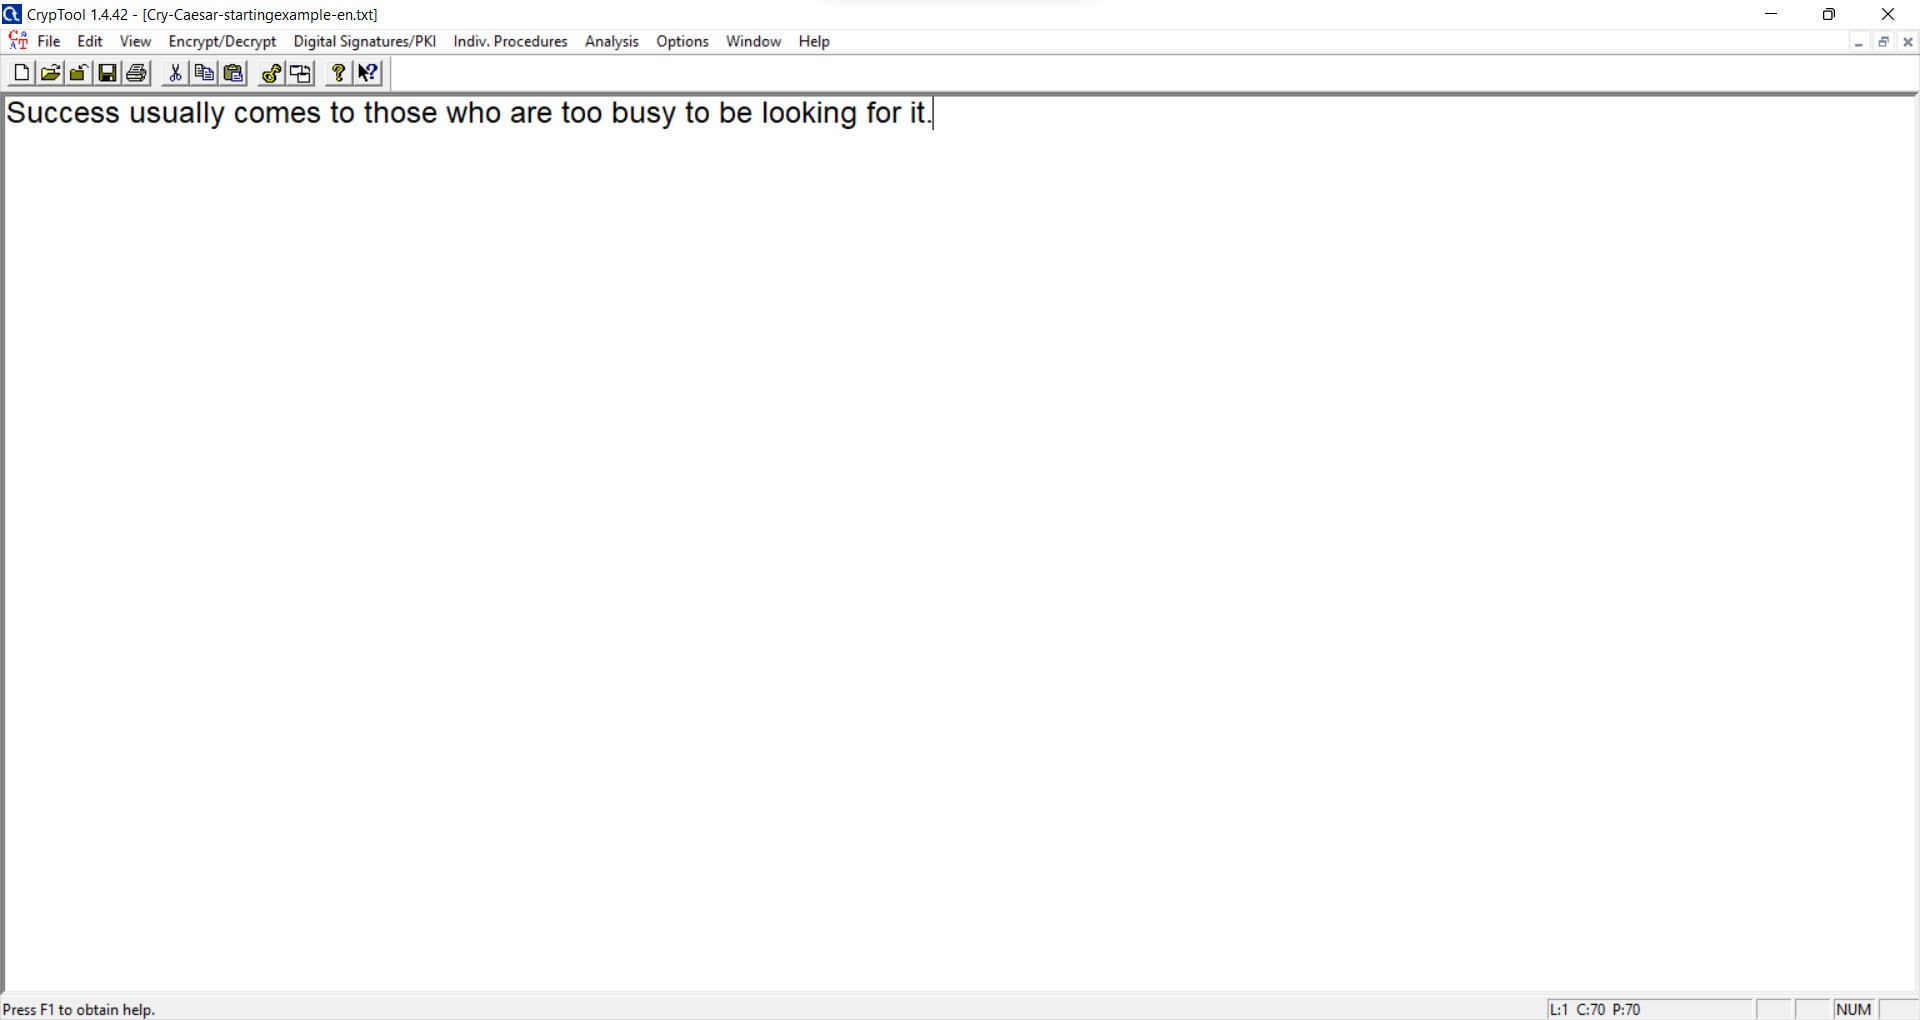
\includegraphics[width=0.75\textwidth]{figures/3ba.jpg}
    \caption
	{}
    \label{fig:fig1}
\end{figure}

\begin{figure}[H]
    \centering
    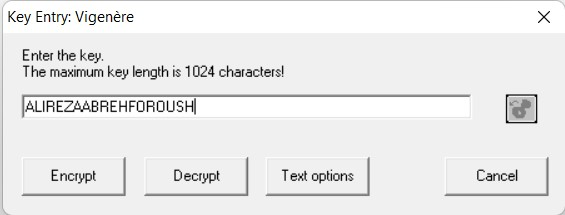
\includegraphics[width=0.25\textwidth]{figures/3bb.jpg}
    \caption
	{}
    \label{fig:fig1}
\end{figure}

\begin{figure}[H]
    \centering
    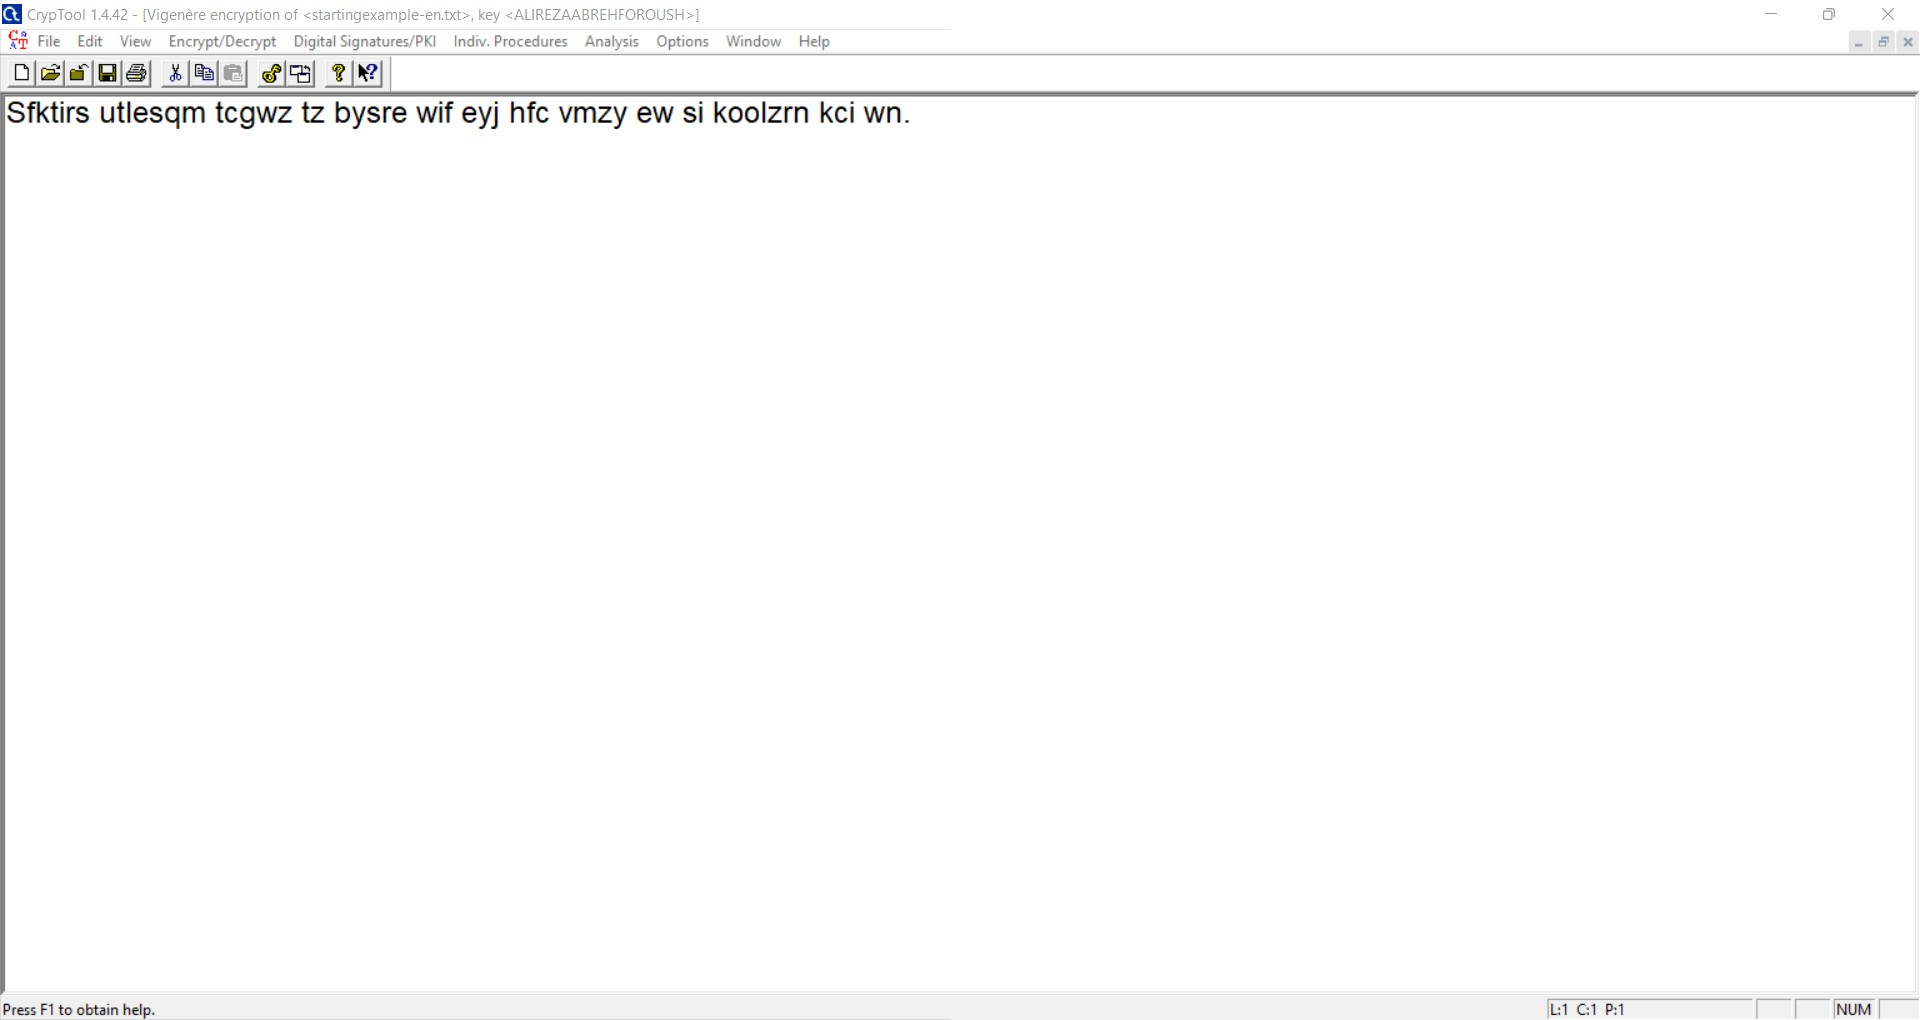
\includegraphics[width=0.75\textwidth]{figures/3bc.jpg}
    \caption
	{}
    \label{fig:fig1}
\end{figure}

\subsection{}
؟؟؟؟؟؟؟؟؟؟؟؟؟؟؟؟؟؟؟؟؟؟؟؟؟؟؟؟؟؟؟؟؟؟؟؟؟؟؟؟؟؟




\section{}%4
در نرم افزار \lr{CrypTool} به صورت زیر رمزگشایی می‌کنیم. طول کلید (به طور پیشفرض) 5 است و کلید در \lr{Vigenère cipher} برابر \lr{SMILE} به دست می‌آید.
\begin{figure}[H]
    \centering
    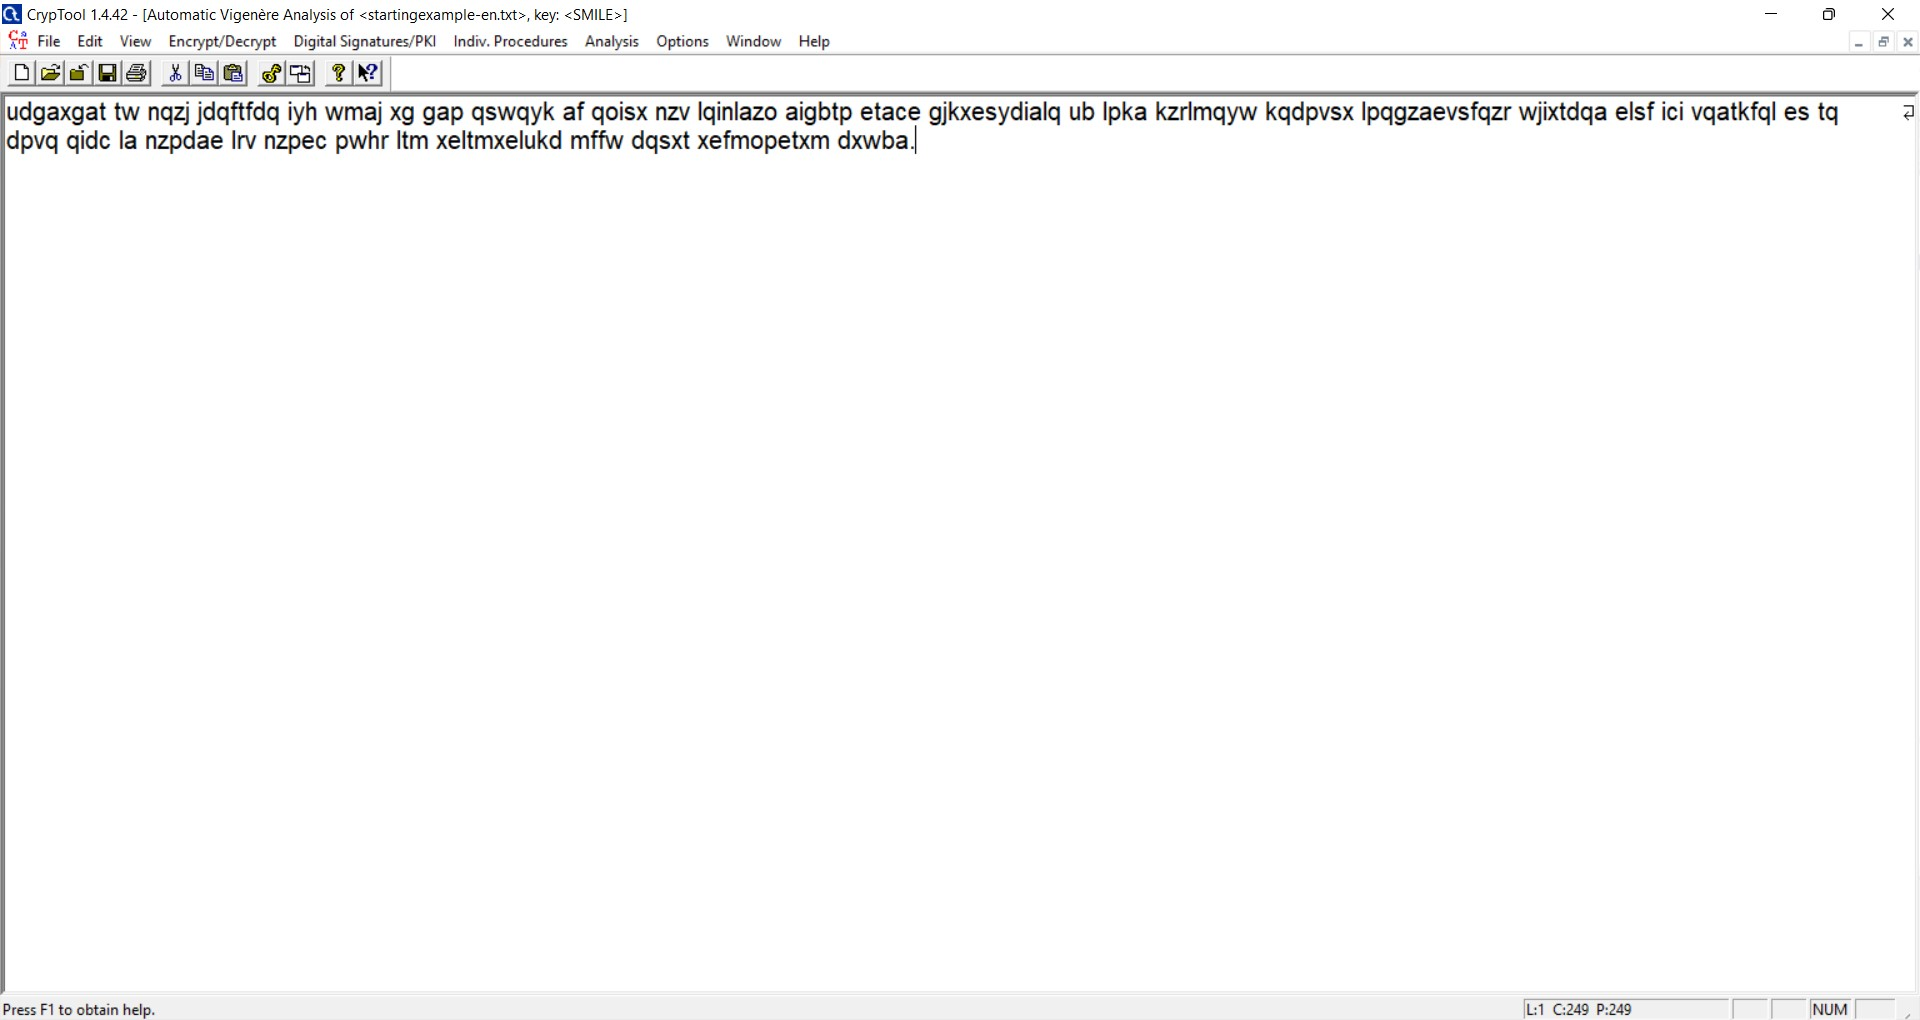
\includegraphics[width=0.75\textwidth]{figures/4a.jpg}
    \caption
	{}
    \label{fig:fig1}
\end{figure}

\begin{figure}[H]
    \centering
    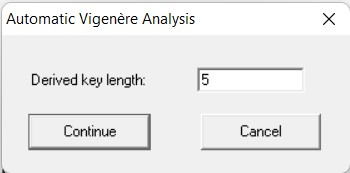
\includegraphics[width=0.25\textwidth]{figures/4b.jpg}
    \caption
	{}
    \label{fig:fig1}
\end{figure}

\begin{figure}[H]
    \centering
    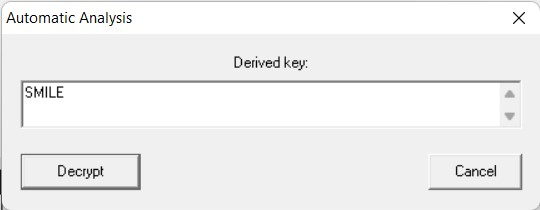
\includegraphics[width=0.25\textwidth]{figures/4c.jpg}
    \caption
	{}
    \label{fig:fig1}
\end{figure}

\begin{figure}[H]
    \centering
    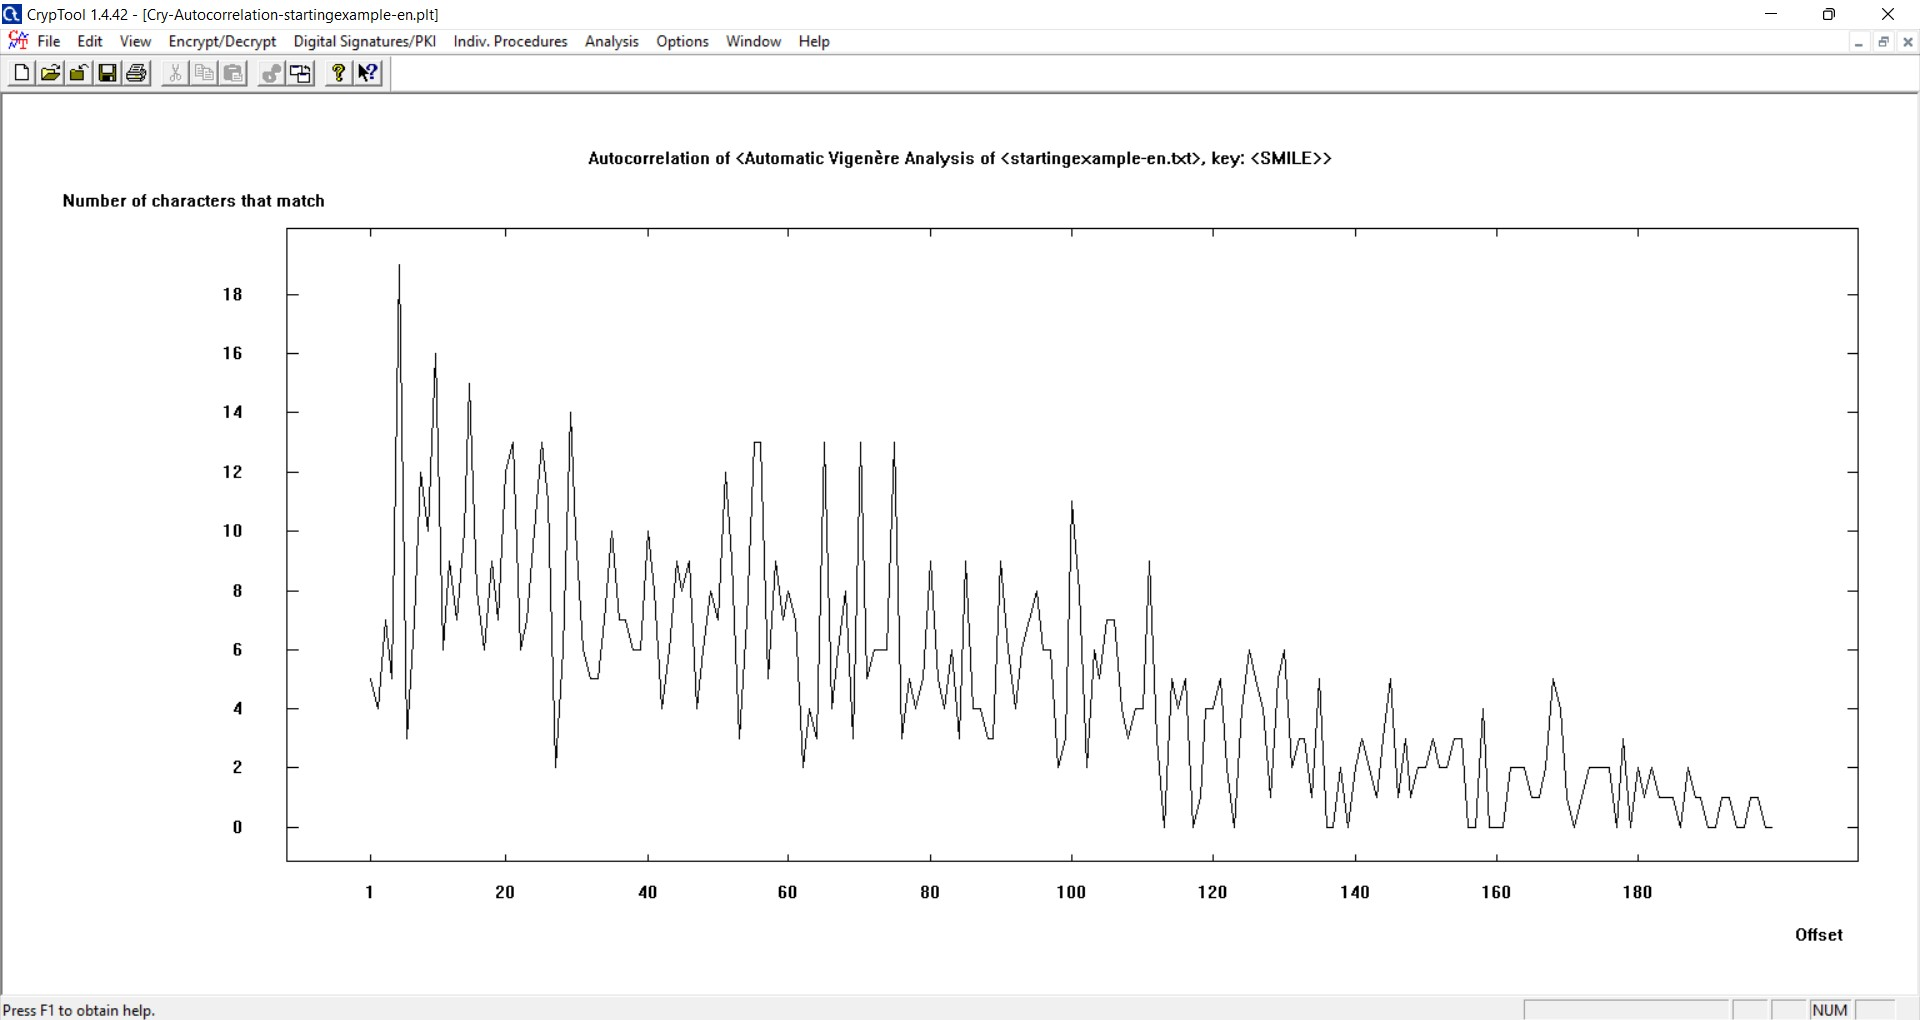
\includegraphics[width=0.75\textwidth]{figures/4d.jpg}
    \caption
	{}
    \label{fig:fig1}
\end{figure}

\begin{figure}[H]
    \centering
    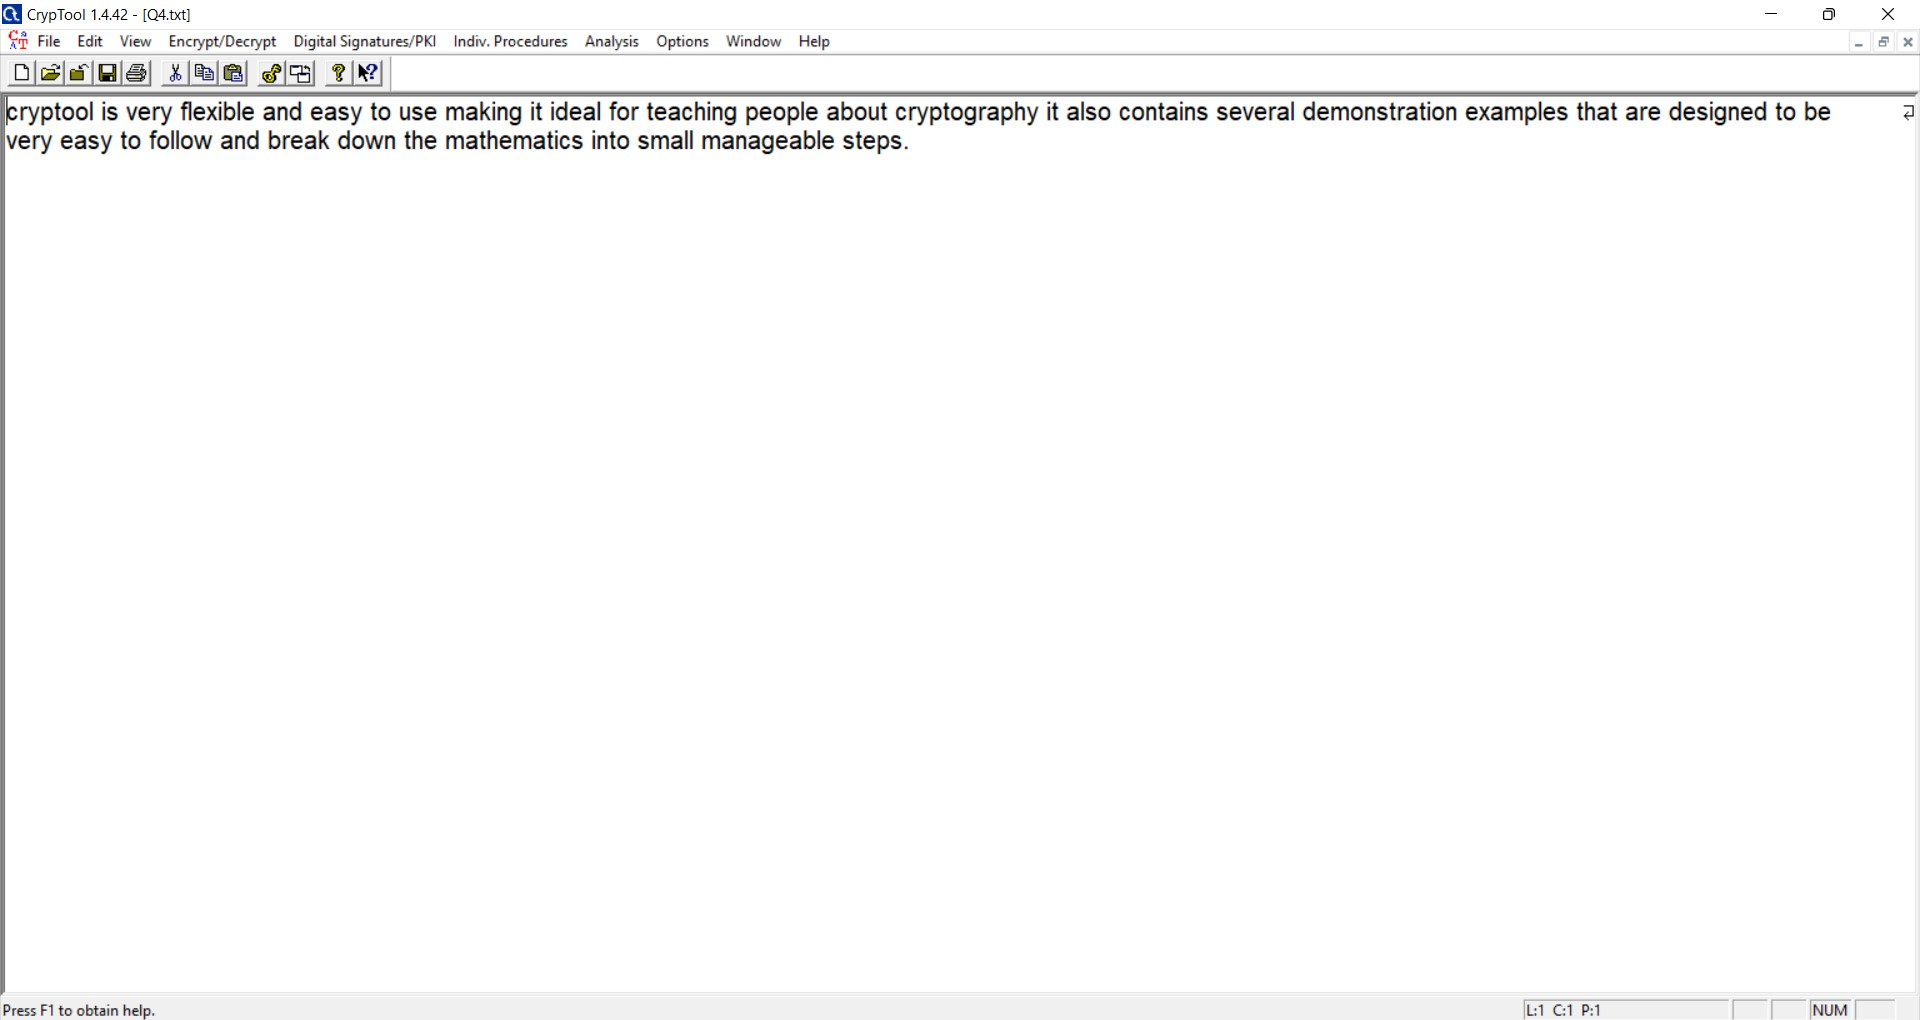
\includegraphics[width=0.75\textwidth]{figures/4e.jpg}
    \caption
	{}
    \label{fig:fig1}
\end{figure}
\lr{autocorrelation} یک متن را با نسخه‌های مختلف شیفت یافته‌ی آن (به طول یکسان) مقایسه می‌کند. در هر حالت کاراکترهایی که باهم \lr{match} می‌شوند (یکسان‌اند) را تعیین می‌کنیم. در نمودار رسم شده، تعداد کاراکترهای \lr{match}شده بر اساس تعداد واحد شیفت داده شده نمایش داده شده است. توجه شود که فقط حروف الفبای انتخاب شده (انگلیسی یا آلمانی برای مثال) تجزیه و تحلیل می‌شوند. همچنین تعداد جابه‌جایی‌ها به طول متن بستگی دارد (شما می‌توانید متنی متشکل از $n$ کاراکتر را حداکثر $n$ واحد جابجا کنید، سپس آن‌ها به نوعی زیر یکدیگر قرار می‌گیرند). به مثال زیر توجه کنید.
\begin{latin}
% Please add the following required packages to your document preamble:
% \usepackage{graphicx}
% \usepackage[table,xcdraw]{xcolor}
% If you use beamer only pass "xcolor=table" option, i.e. \documentclass[xcolor=table]{beamer}
\begin{table}[H]
\centering
\resizebox{\columnwidth}{!}{%
\begin{tabular}{|c|c|c|c|c|c|c|c|c|c|c|c|c|c|c|c|c|c|c|c|c|c|c|c|c|c|c|c|c|c|c|c|c|c|c|c|c|c|c|c|c|c|c|c|c|c|c|c|c|c|c|c|c|c|c|c|c|c|c|c|c|c|c|c|c|c|c|c|c|c|llllll}
\cline{1-70}
Orginal text & S & u & c & c & e & s & s                                  &                                    & u          & s & u & a & l & l & y &   & c & o & m & e & s &   & t & o &                                    & t & h & o & s & e &   & w                                  & h & o &                                    & a & r & e &   & t & o                                  & o                                  &   & b & u & s & y &   & t & o &   & b                                  & e &            & l & o & o & k & i & n & g &   & f & o & r &  & i & t & . &                      &                      &                      &                      &                      &                      \\ \cline{1-70}
Modified     & S & u & c & c & e & s & \cellcolor[HTML]{FFCCC9}\textbf{s} & \cellcolor[HTML]{FFCCC9}\textbf{u} & \textbf{s} & u & a & l & l & y & c & o & m & e & s & t & o & t & h & o & \cellcolor[HTML]{FFCCC9}\textbf{s} & e & w & h & o & a & r & \cellcolor[HTML]{FFCCC9}\textbf{e} & t & o & \cellcolor[HTML]{FFCCC9}\textbf{o} & b & u & s & y & t & \cellcolor[HTML]{FFCCC9}\textbf{o} & \cellcolor[HTML]{FFCCC9}\textbf{b} & e & l & o & o & k & i & n & g & f & \cellcolor[HTML]{FFCCC9}\textbf{o} & r & \textbf{i} & t & . &   &   &   &   &   &   &   &   &   &  &   &   &   &                      &                      &                      &                      &                      &                      \\ \cline{1-70}
Shifted by 6 &   &   &   &   &   &   & \cellcolor[HTML]{FFCCC9}\textbf{S} & \cellcolor[HTML]{FFCCC9}\textbf{u} & c          & c & e & s & s & u & s & u & a & l & l & y & c & o & m & e & \cellcolor[HTML]{FFCCC9}\textbf{s} & t & o & t & h & o & s & \cellcolor[HTML]{FFCCC9}\textbf{e} & w & h & \cellcolor[HTML]{FFCCC9}\textbf{o} & a & r & e & t & o & \cellcolor[HTML]{FFCCC9}\textbf{o} & \cellcolor[HTML]{FFCCC9}\textbf{b} & u & s & y & t & o & b & e & l & o & \cellcolor[HTML]{FFCCC9}\textbf{o} & k & \textbf{i} & n & g & f & o & r & i & t & . &   &   &   &  &   &   &   & \multicolumn{1}{c}{} & \multicolumn{1}{c}{} & \multicolumn{1}{c}{} & \multicolumn{1}{c}{} & \multicolumn{1}{c}{} & \multicolumn{1}{c}{} \\ \cline{1-70}
\end{tabular}%
}
\end{table}
\end{latin}
در این مثال در شیفت 6 واحد، تعداد کاراکترهای \lr{match}شده برابر 8 است.


%\begin{latin}
%\lstinputlisting{sources/p2.m}
%\end{latin}


%%%%%%%%%%%%%%%%%%%%%%%%%%%%%%%%%%%
%%%%%%%%%%%%%%%%%%%%%%%%%%%%%%%%%%%
%%%%%%%%%%%%%%%%%%%%%%%%%%%%%%%%%%%

%------------------------------------------------------------------------------------------


\section*{منابع}
\renewcommand{\section}[2]{}%
\begin{thebibliography}{99} % assumes less than 100 references
%چنانچه مرجع فارسی نیز داشته باشید باید دستور فوق را فعال کنید و مراجع فارسی خود را بعد از این دستور وارد کنید


\begin{LTRitems}

\resetlatinfont

\bibitem{b1}
\end{LTRitems}

\end{thebibliography}


\end{document}
